\PassOptionsToPackage{unicode=true}{hyperref} % options for packages loaded elsewhere
\PassOptionsToPackage{hyphens}{url}
%
\documentclass[]{article}
\usepackage{lmodern}
\usepackage{amssymb,amsmath}
\usepackage{ifxetex,ifluatex}
\usepackage{fixltx2e} % provides \textsubscript
\ifnum 0\ifxetex 1\fi\ifluatex 1\fi=0 % if pdftex
  \usepackage[T1]{fontenc}
  \usepackage[utf8]{inputenc}
  \usepackage{textcomp} % provides euro and other symbols
\else % if luatex or xelatex
  \usepackage{unicode-math}
  \defaultfontfeatures{Ligatures=TeX,Scale=MatchLowercase}
    \setmainfont[]{Carlito}
\fi
% use upquote if available, for straight quotes in verbatim environments
\IfFileExists{upquote.sty}{\usepackage{upquote}}{}
% use microtype if available
\IfFileExists{microtype.sty}{%
\usepackage[]{microtype}
\UseMicrotypeSet[protrusion]{basicmath} % disable protrusion for tt fonts
}{}
\IfFileExists{parskip.sty}{%
\usepackage{parskip}
}{% else
\setlength{\parindent}{0pt}
\setlength{\parskip}{6pt plus 2pt minus 1pt}
}
\usepackage{hyperref}
\hypersetup{
            pdftitle={Diagnostic IDEA4},
            pdfborder={0 0 0},
            breaklinks=true}
\urlstyle{same}  % don't use monospace font for urls
\usepackage[margin=1in]{geometry}
\usepackage{longtable,booktabs}
% Fix footnotes in tables (requires footnote package)
\IfFileExists{footnote.sty}{\usepackage{footnote}\makesavenoteenv{longtable}}{}
\usepackage{graphicx,grffile}
\makeatletter
\def\maxwidth{\ifdim\Gin@nat@width>\linewidth\linewidth\else\Gin@nat@width\fi}
\def\maxheight{\ifdim\Gin@nat@height>\textheight\textheight\else\Gin@nat@height\fi}
\makeatother
% Scale images if necessary, so that they will not overflow the page
% margins by default, and it is still possible to overwrite the defaults
% using explicit options in \includegraphics[width, height, ...]{}
\setkeys{Gin}{width=\maxwidth,height=\maxheight,keepaspectratio}
\setlength{\emergencystretch}{3em}  % prevent overfull lines
\providecommand{\tightlist}{%
  \setlength{\itemsep}{0pt}\setlength{\parskip}{0pt}}
\setcounter{secnumdepth}{5}
% Redefines (sub)paragraphs to behave more like sections
\ifx\paragraph\undefined\else
\let\oldparagraph\paragraph
\renewcommand{\paragraph}[1]{\oldparagraph{#1}\mbox{}}
\fi
\ifx\subparagraph\undefined\else
\let\oldsubparagraph\subparagraph
\renewcommand{\subparagraph}[1]{\oldsubparagraph{#1}\mbox{}}
\fi

% set default figure placement to htbp
\makeatletter
\def\fps@figure{htbp}
\makeatother

\usepackage[french]{babel}
\usepackage{lastpage}
\usepackage{float}
\usepackage{graphicx}
\usepackage{caption}
\usepackage{tocloft}
\renewcommand\cftsecfont{\Large}
\renewcommand\cftsubsecfont{\large}
\renewcommand\cftsubsubsecfont{\large}
\renewcommand\cftsecpagefont{\Large}
\captionsetup[figure]{font=large}
\usepackage{fancyhdr}
\pagestyle{fancy}
\fancyfoot[C]{Diagnostic IDEA4 - 10 janvier 2020}
\fancyfoot[R]{Page \thepage / \pageref{LastPage}}
\usepackage{etoolbox}
\makeatletter
\providecommand{\subtitle}[1]{% add subtitle to \maketitle
  \apptocmd{\@title}{\par {\large #1 \par}}{}{}
}
\makeatother

\title{Diagnostic IDEA4}
\providecommand{\subtitle}[1]{}
\subtitle{Eléments de sortie d'analyse individuelle - Version 0.1}
\author{}
\date{\vspace{-2.5em}10 janvier 2020}

\begin{document}
\maketitle

{
\setcounter{tocdepth}{3}
\tableofcontents
}
\fancyfoot[L]{Exploitation : Michel GALMEL}

\vspace{+3cm}
\Large

\begin{longtable}[]{@{}ll@{}}
\toprule
\endhead
NOM Prénom : & Michel GALMEL\tabularnewline
Département : & Eure\tabularnewline
Type d'exploitation : & Grande culture, agroforesterie, permaculture,
accueil\tabularnewline
Forme sociétaire : & Individuel\tabularnewline
SAU (hors forêt) : & 61\tabularnewline
\bottomrule
\end{longtable}

\newpage

\hypertarget{lecture-par-les-dimensions}{%
\section{Lecture par les dimensions}\label{lecture-par-les-dimensions}}

\hypertarget{ruxe9sultats-pour-les-dimensions}{%
\subsection{Résultats pour les
dimensions}\label{ruxe9sultats-pour-les-dimensions}}

\Large

La note d'IDEA4 obtenue pour cette exploitation est de \textbf{45 /
100}.

\large

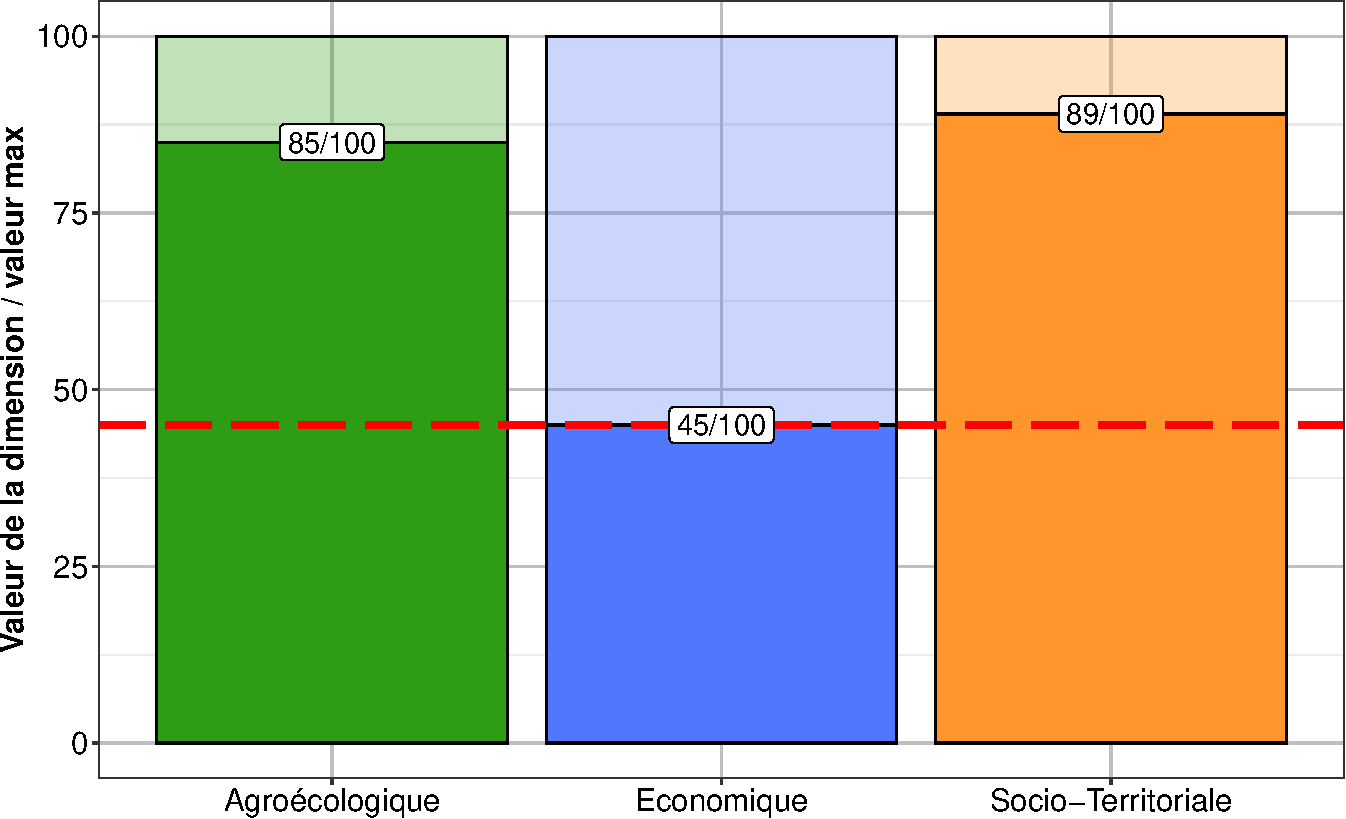
\includegraphics[width=1\linewidth]{report_files/figure-latex/unnamed-chunk-4-1}

\hypertarget{ruxe9sultats-pour-les-composantes}{%
\subsection{Résultats pour les
composantes}\label{ruxe9sultats-pour-les-composantes}}

\begin{figure}[H]
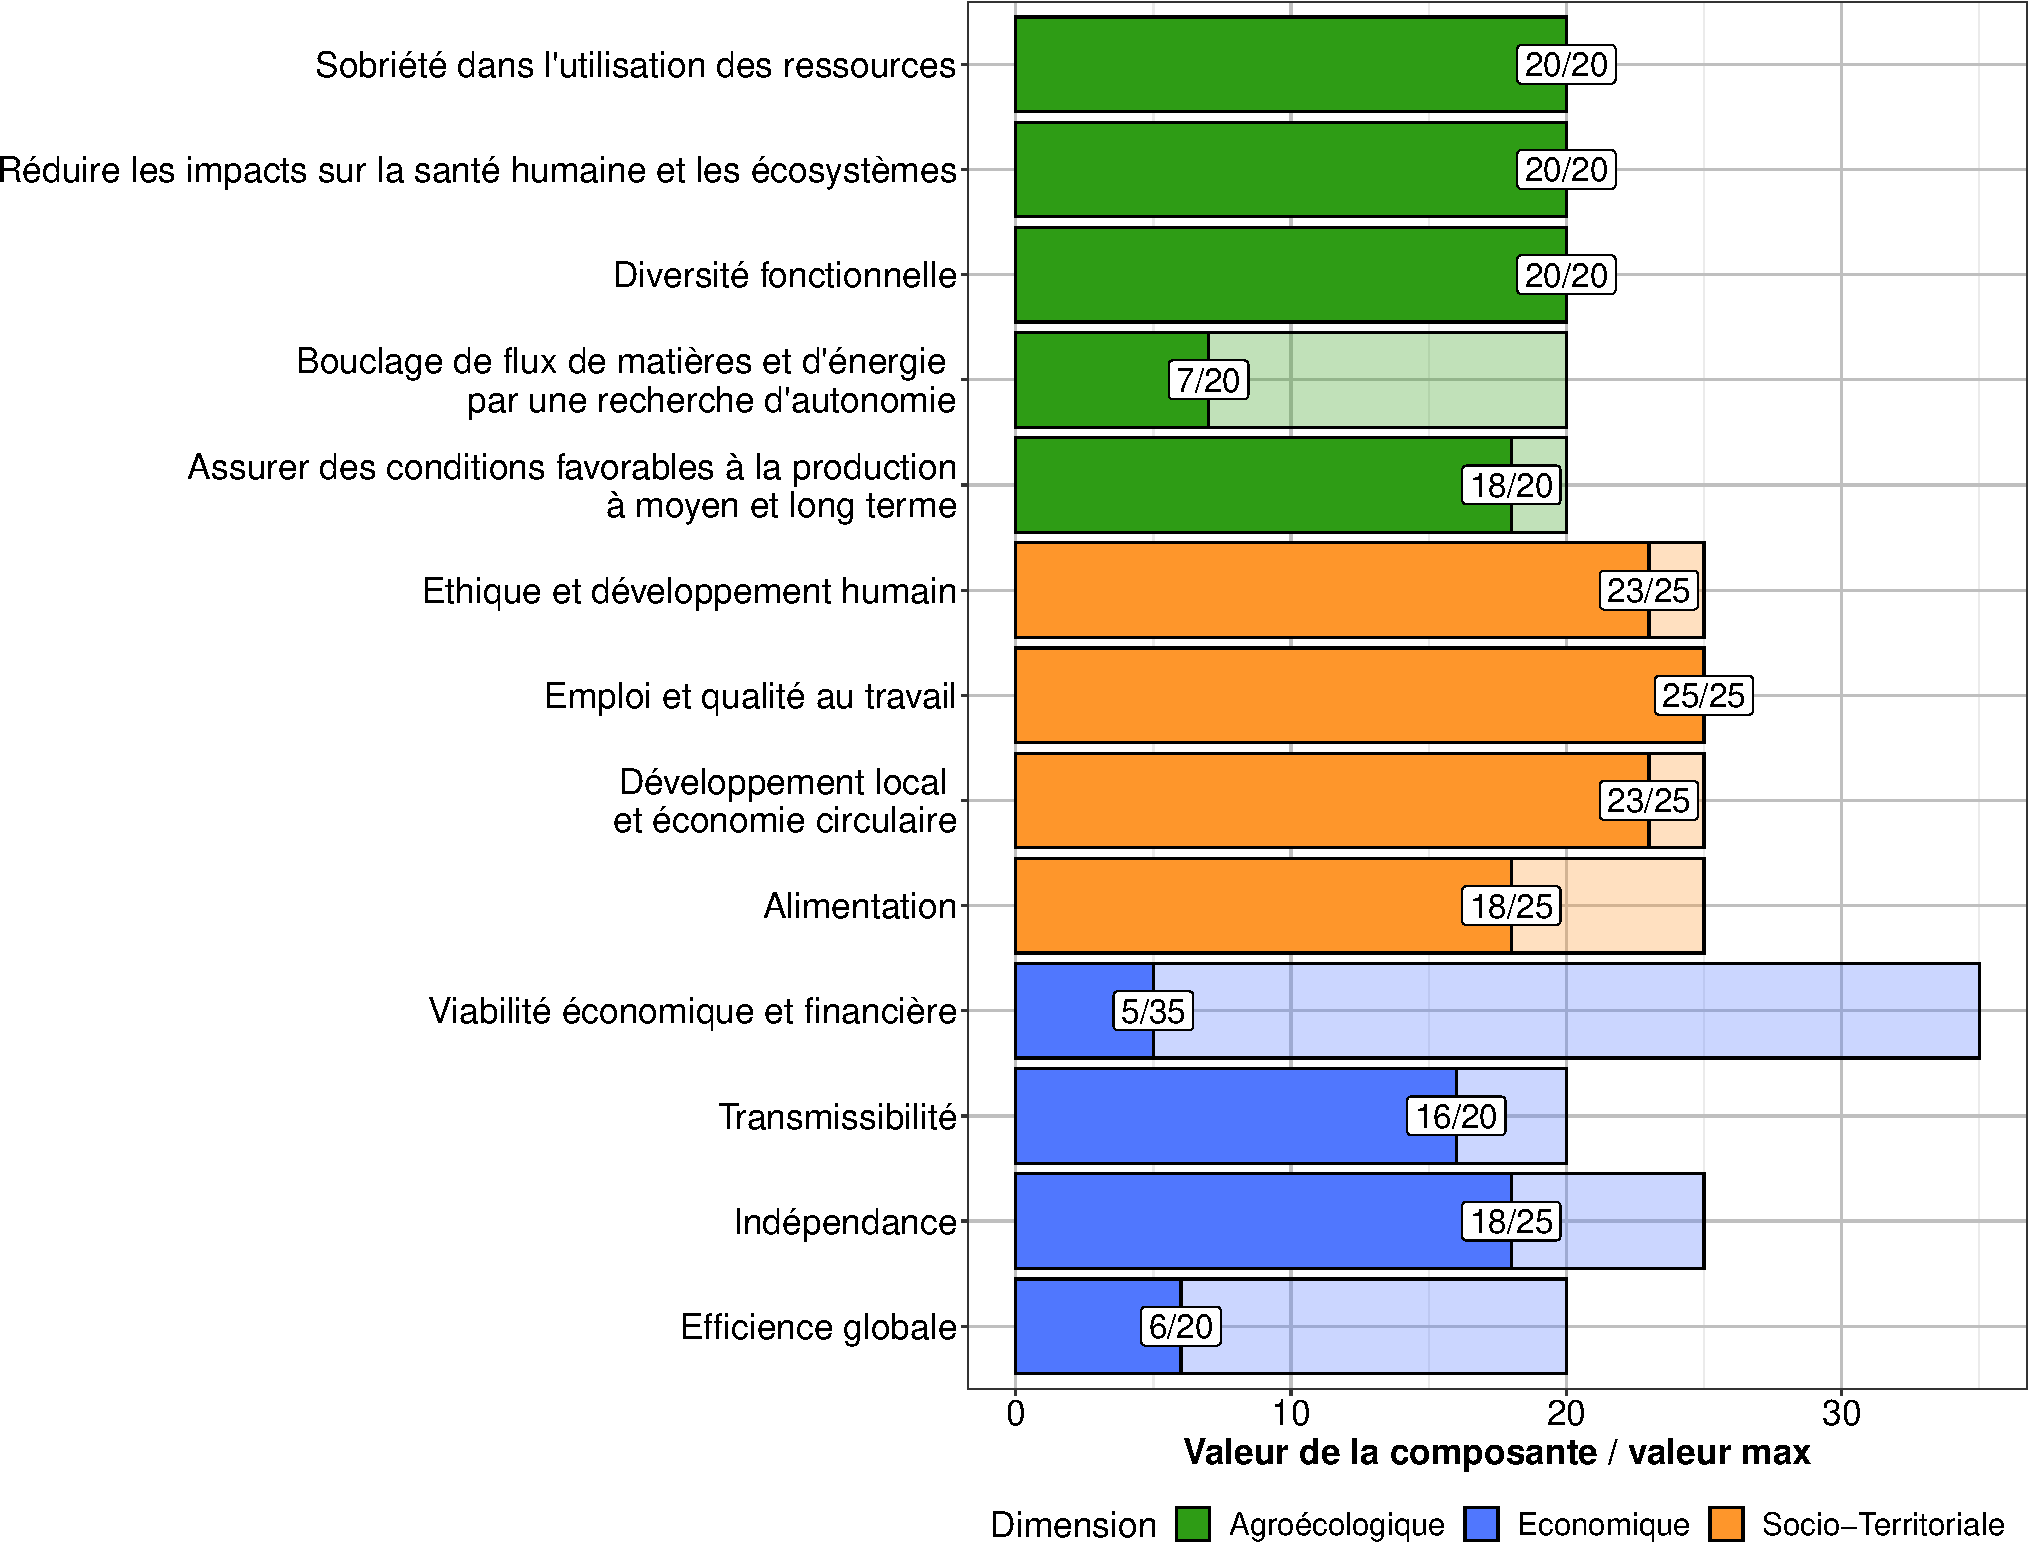
\includegraphics[width=1\linewidth]{report_files/figure-latex/unnamed-chunk-5-1} \caption{Composantes}\label{fig:unnamed-chunk-5}
\end{figure}

\hypertarget{ruxe9sultats-pour-les-indicateurs}{%
\subsection{Résultats pour les
indicateurs}\label{ruxe9sultats-pour-les-indicateurs}}

\hypertarget{indicateurs-agroecologiques}{%
\subsubsection{Indicateurs
AgroEcologiques}\label{indicateurs-agroecologiques}}

\begin{figure}[H]
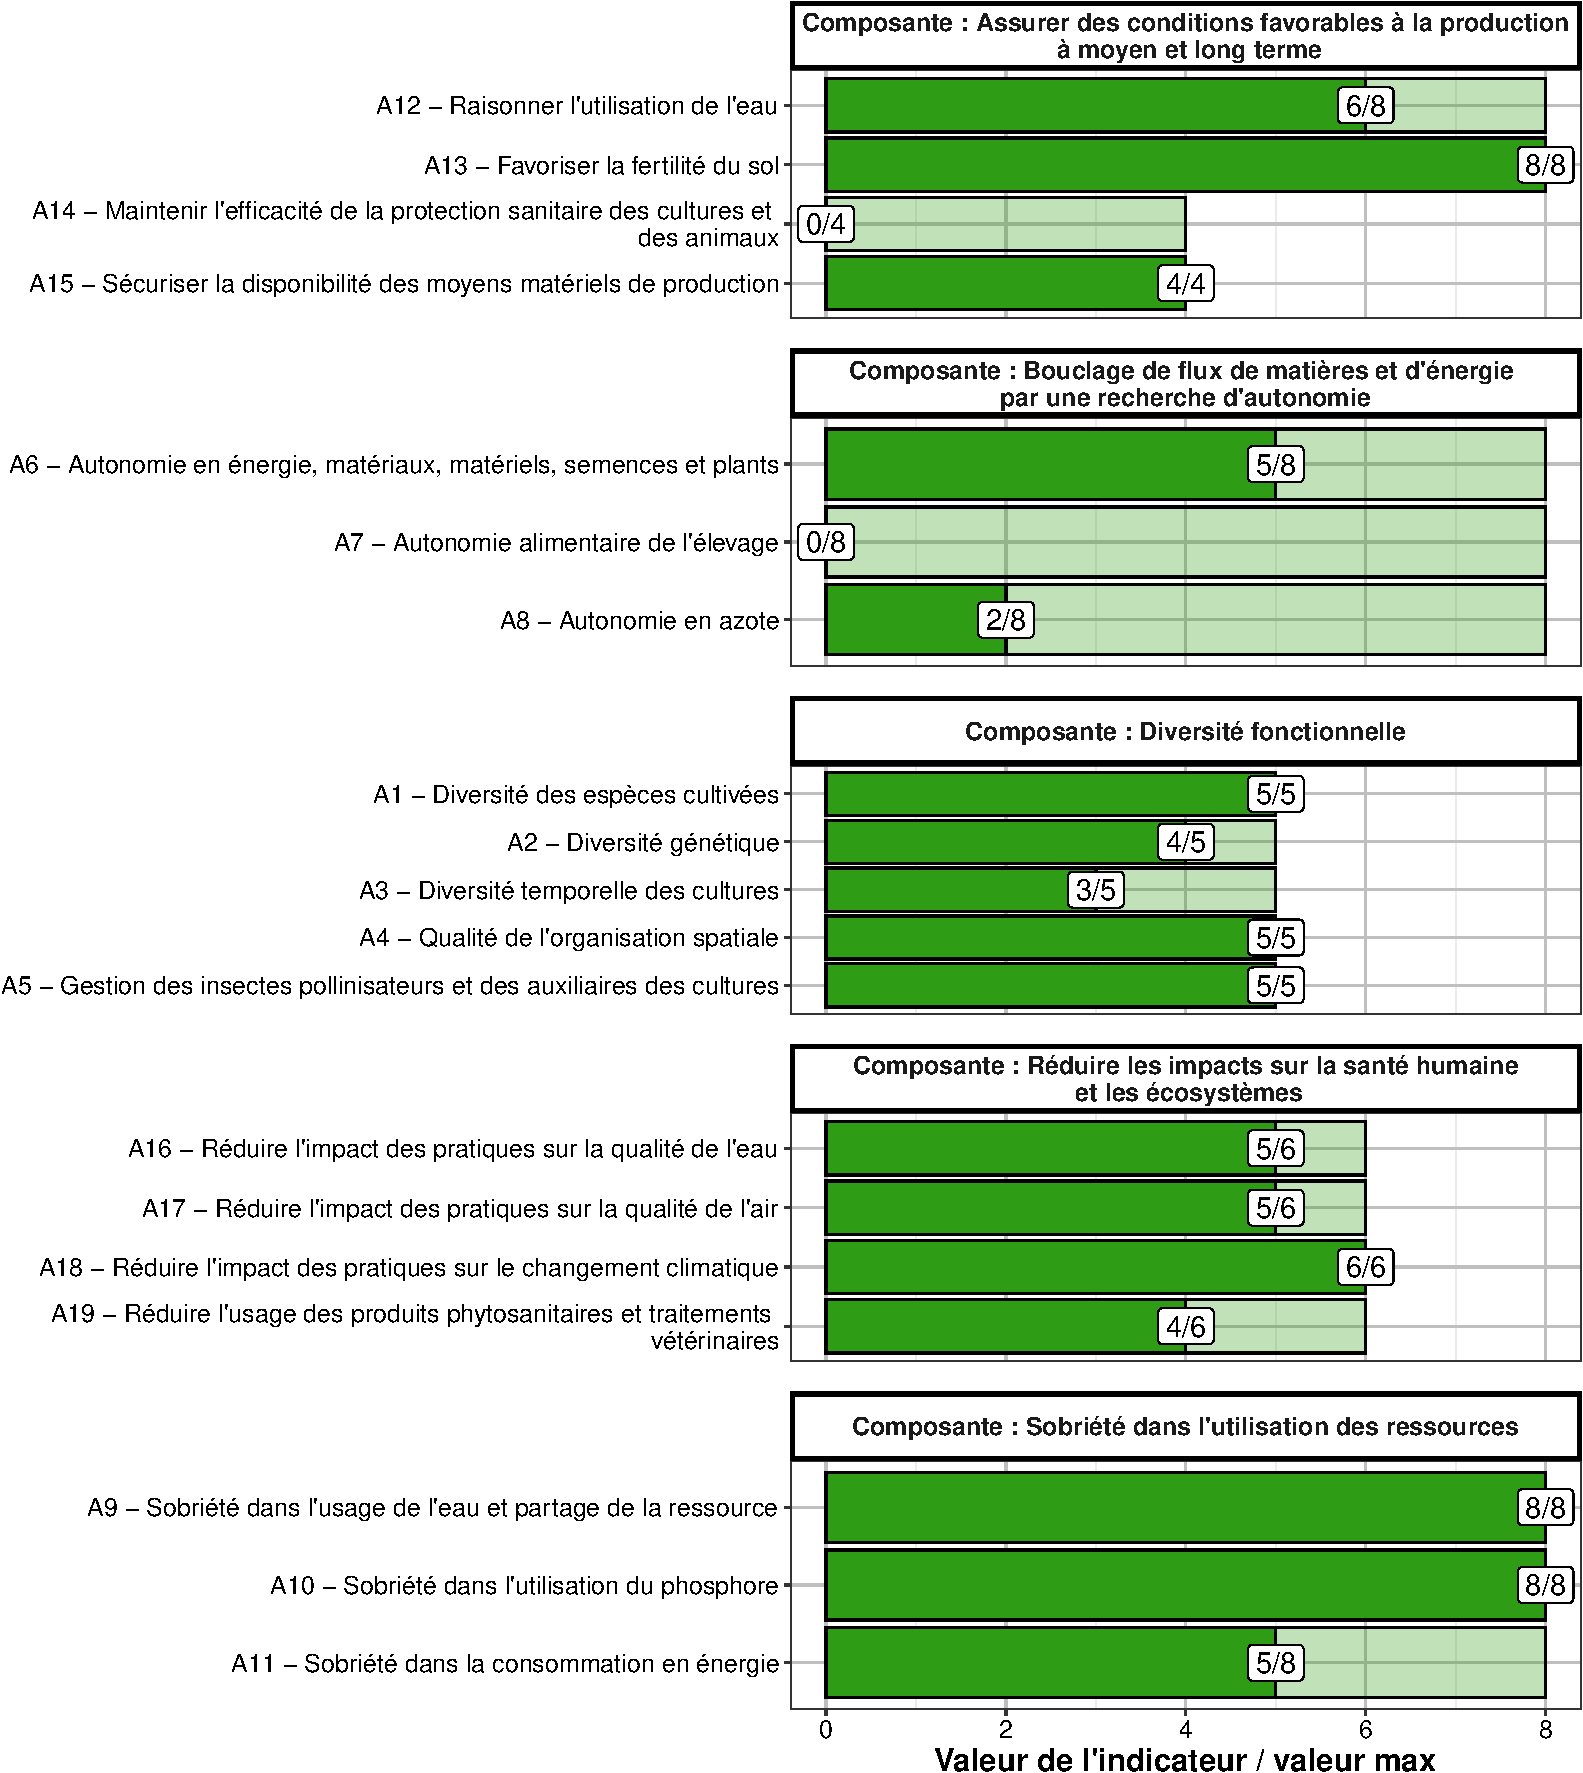
\includegraphics[width=1\linewidth]{report_files/figure-latex/unnamed-chunk-6-1} \caption{Indicateurs AgroEcologiques}\label{fig:unnamed-chunk-6}
\end{figure}

\hypertarget{indicateurs-socio-territoriaux}{%
\subsubsection{Indicateurs
Socio-Territoriaux}\label{indicateurs-socio-territoriaux}}

\begin{figure}[H]
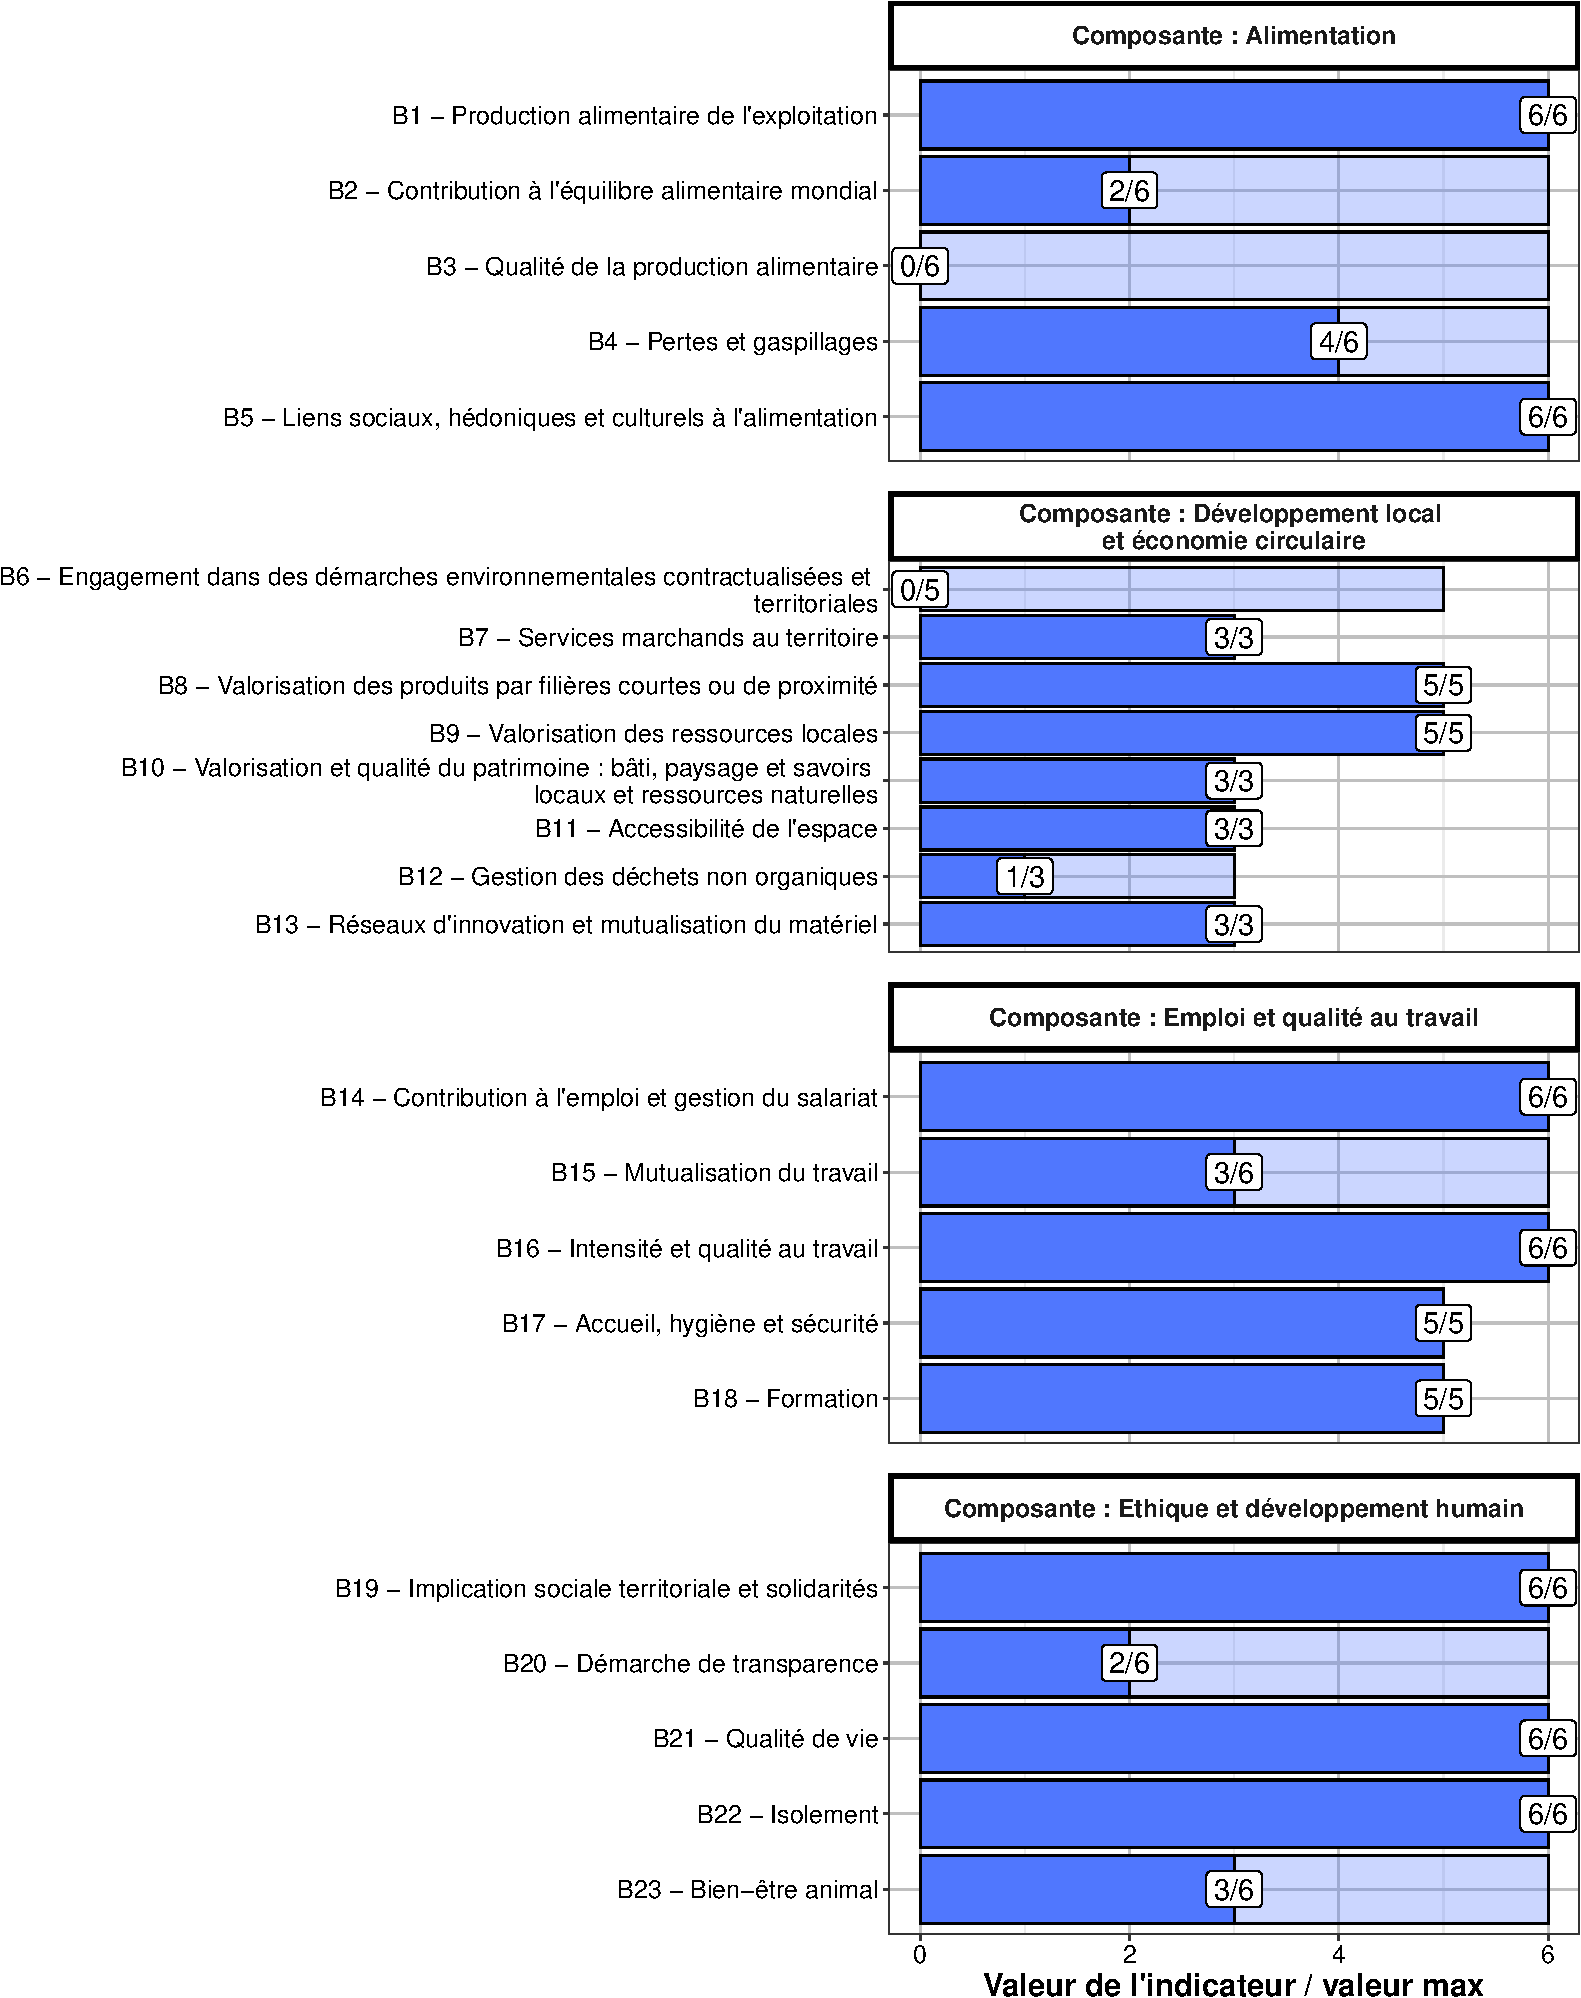
\includegraphics[width=1\linewidth]{report_files/figure-latex/unnamed-chunk-7-1} \caption{Indicateurs socio-territoriaux}\label{fig:unnamed-chunk-7}
\end{figure}

\hypertarget{indicateurs-economiques}{%
\subsubsection{Indicateurs Economiques}\label{indicateurs-economiques}}

\begin{figure}[H]
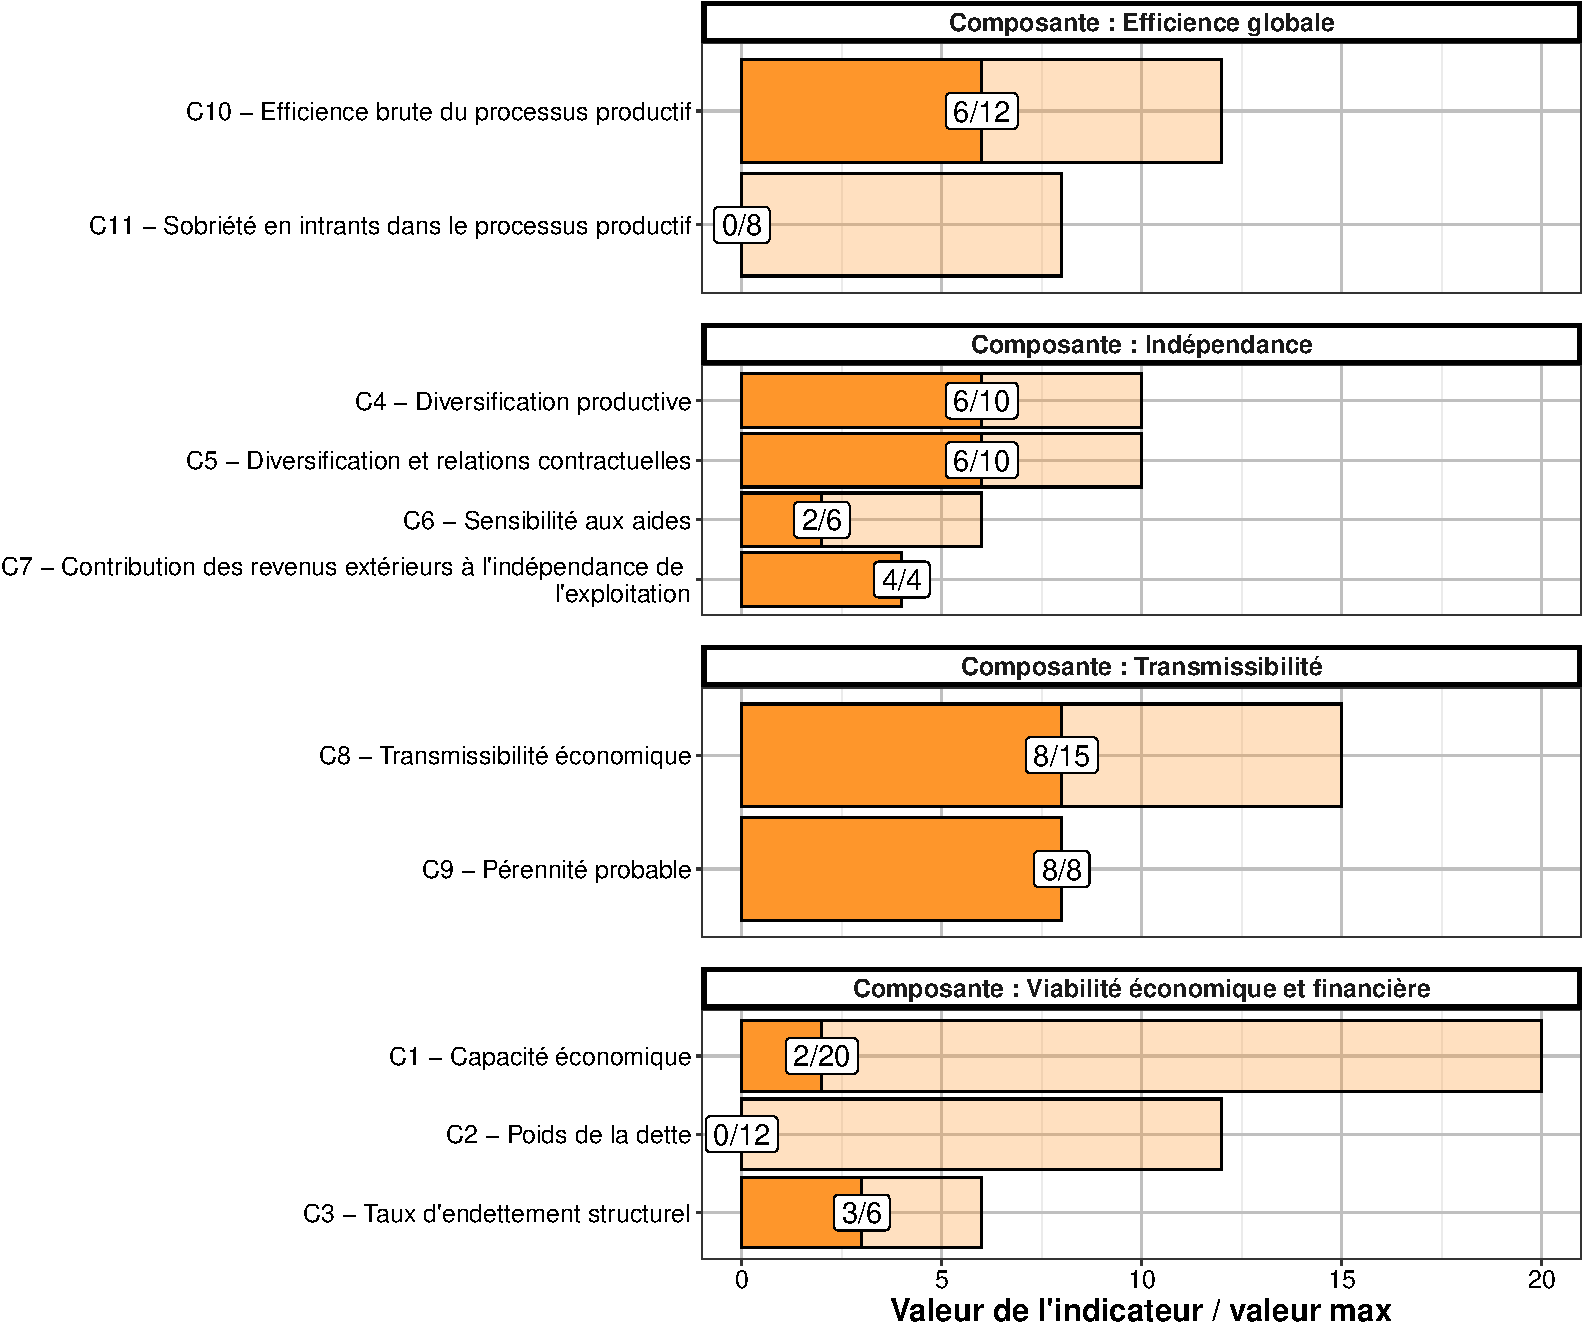
\includegraphics[width=1\linewidth]{report_files/figure-latex/unnamed-chunk-8-1} \caption{Indicateurs Economiques}\label{fig:unnamed-chunk-8}
\end{figure}

\hbox{}

\hypertarget{lecture-par-les-propriuxe9tuxe9s}{%
\section{Lecture par les
propriétés}\label{lecture-par-les-propriuxe9tuxe9s}}

\hypertarget{arbres-uxe9clairuxe9-des-propriuxe9tuxe9s}{%
\subsection{Arbres éclairé des
propriétés}\label{arbres-uxe9clairuxe9-des-propriuxe9tuxe9s}}

\rotatebox{270}{

\begin{minipage}{0.85\textheight}


\begin{figure}[H]
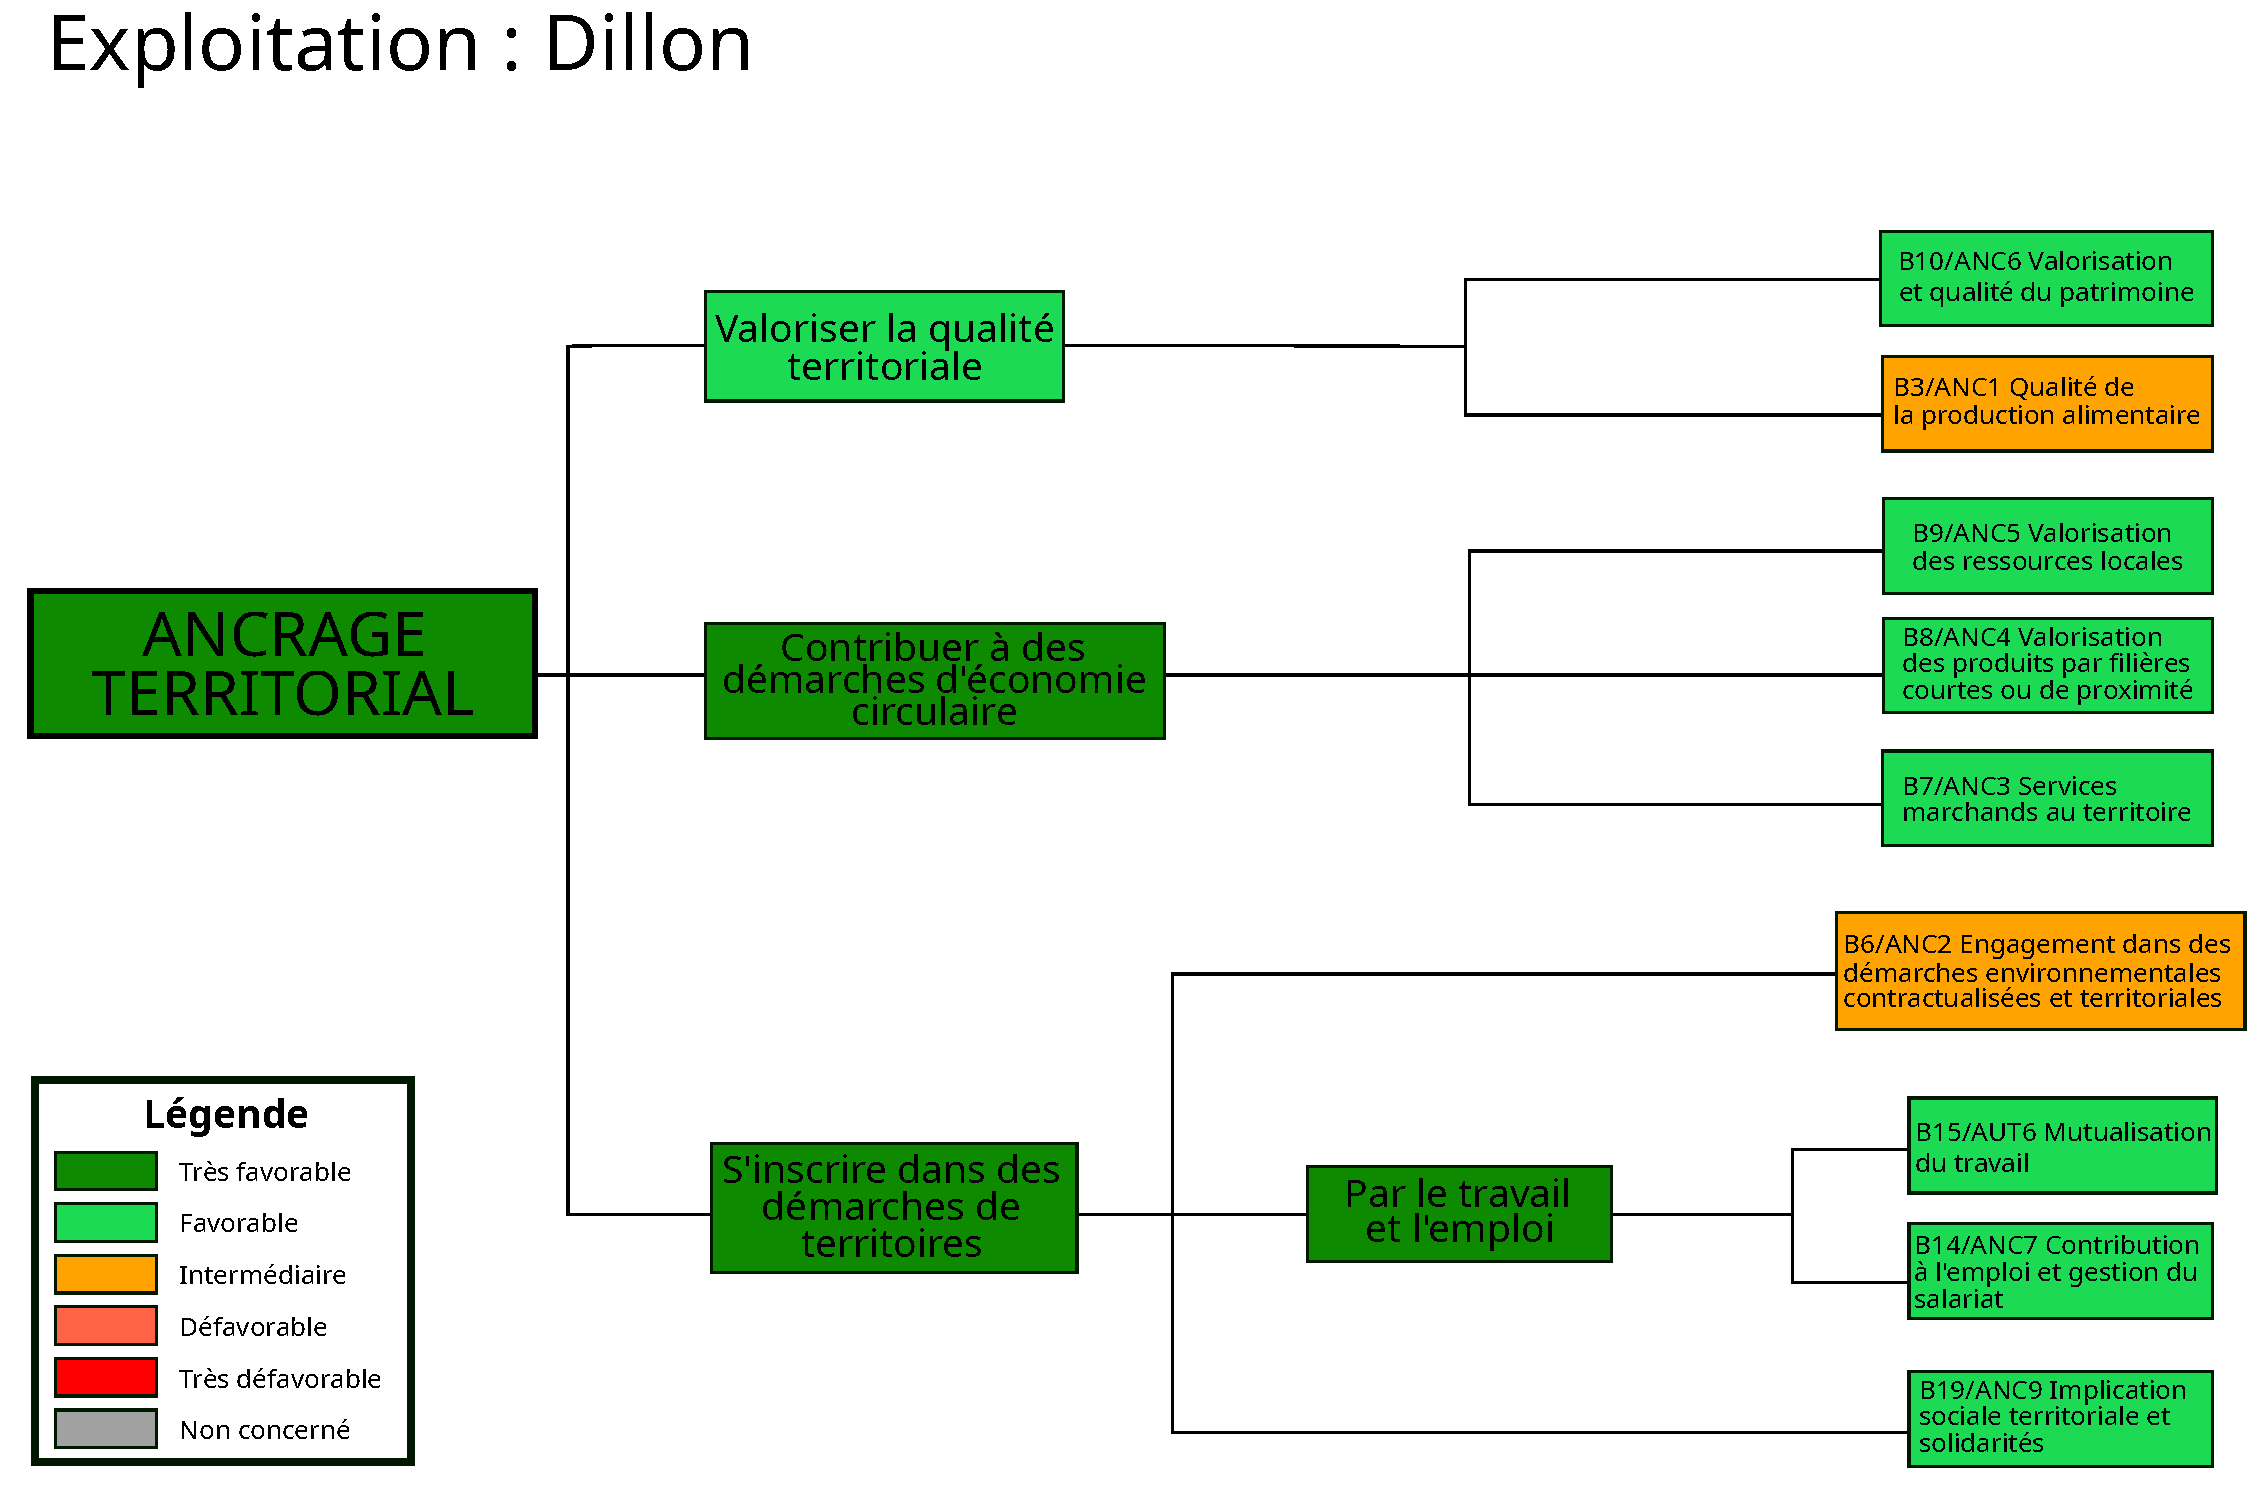
\includegraphics[width=1\linewidth]{/tmp/Rtmpy9IFHR/Michel_GALMEL/Propriétés/Cartes_heuristiques/Ancrage} \caption{Ancrage territorial}\label{fig:unnamed-chunk-10}
\end{figure}

\end{minipage}}

\rotatebox{270}{
\begin{minipage}{\textheight}
\begin{figure}[H]
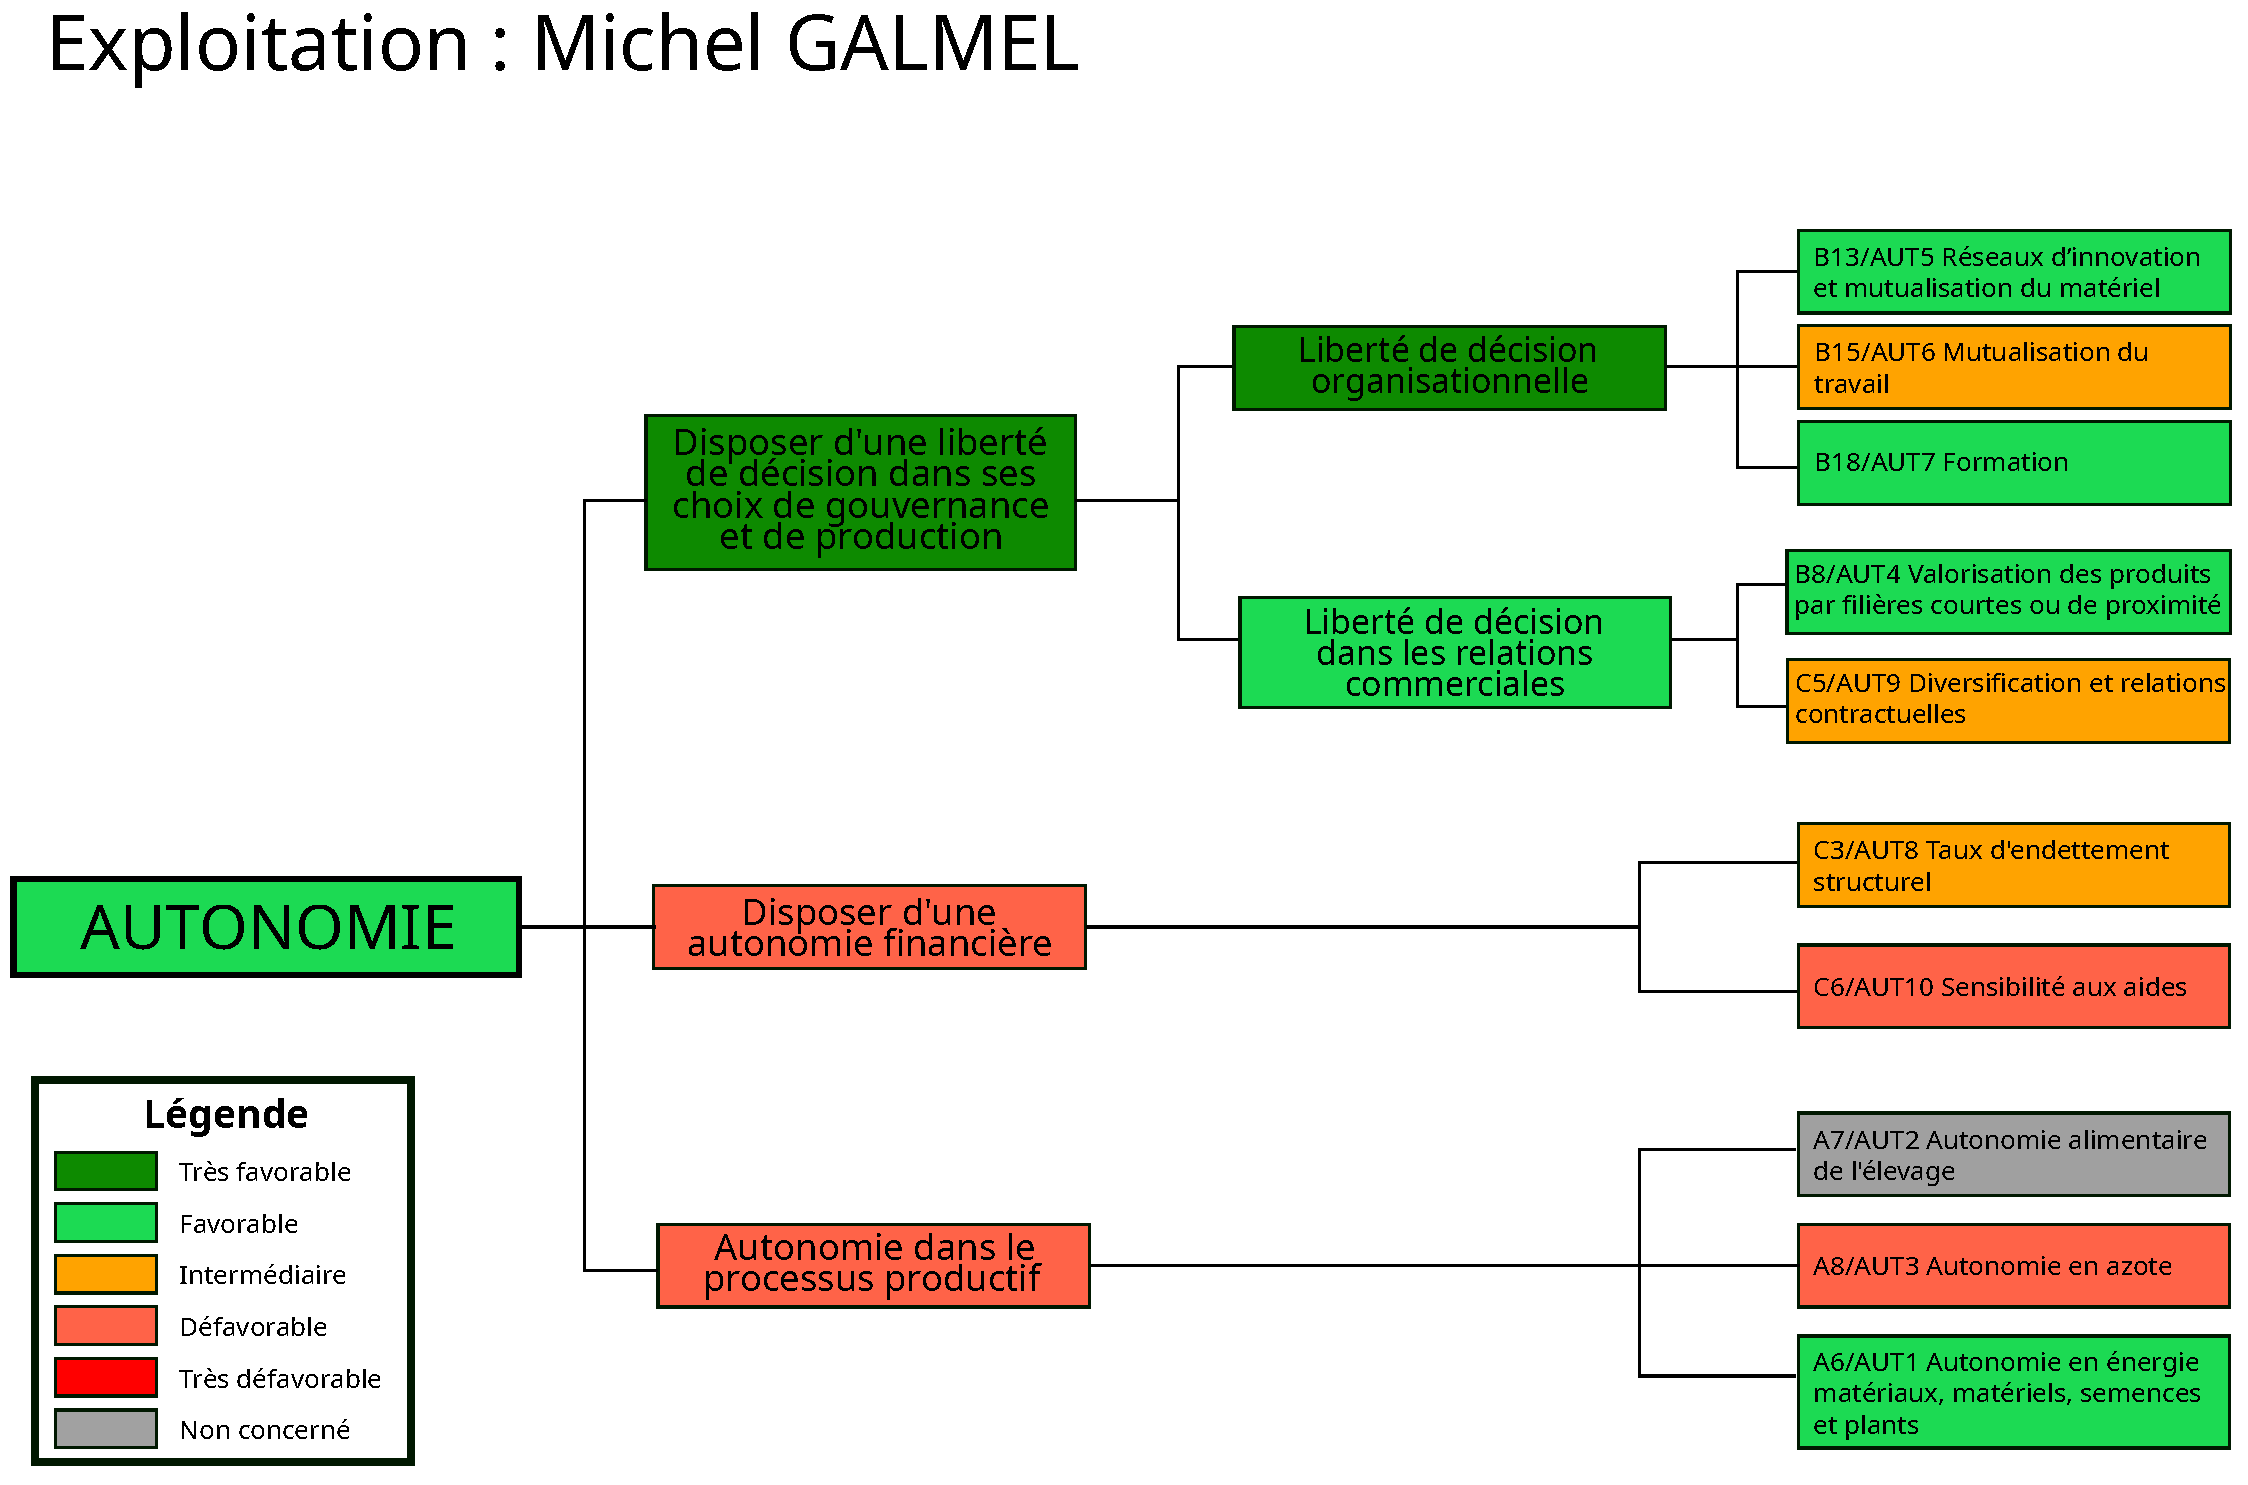
\includegraphics[width=1\linewidth]{/tmp/Rtmpy9IFHR/Michel_GALMEL/Propriétés/Cartes_heuristiques/Autonomie} \caption{Autonomie}\label{fig:unnamed-chunk-11}
\end{figure}
\end{minipage}}

\rotatebox{270}{
\begin{minipage}{\textheight}
\begin{figure}[H]
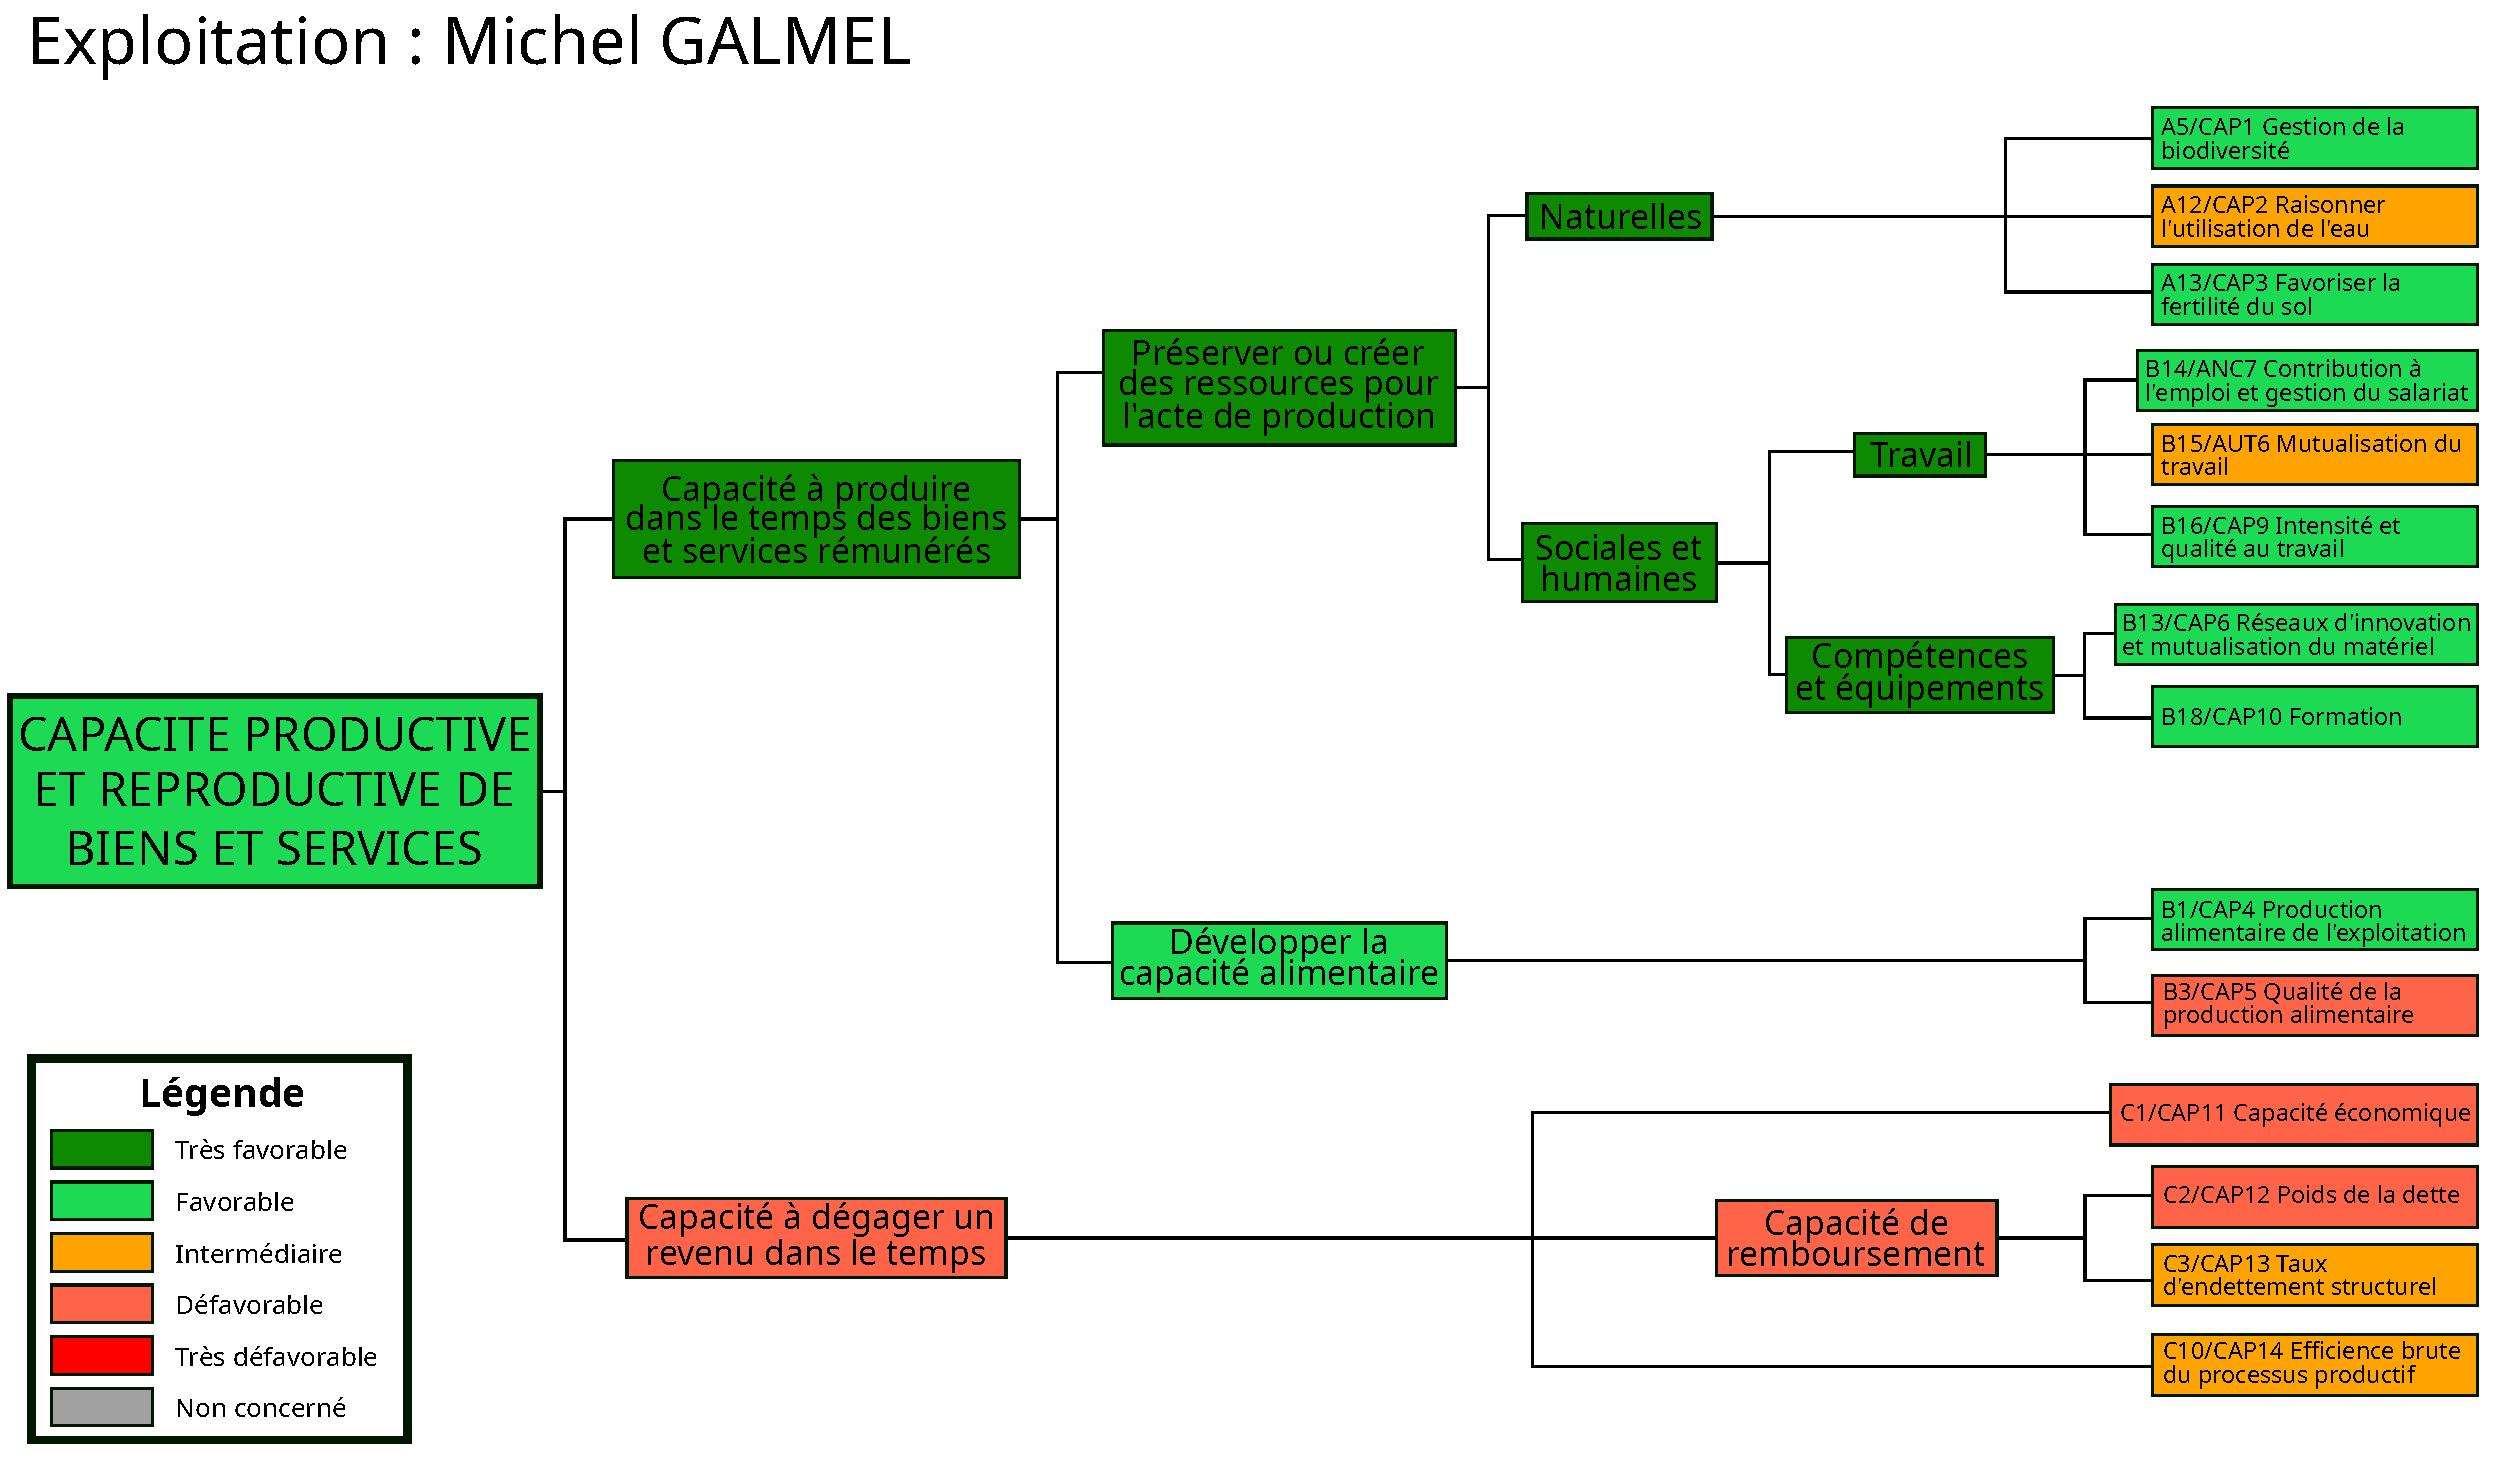
\includegraphics[width=1\linewidth]{/tmp/Rtmpy9IFHR/Michel_GALMEL/Propriétés/Cartes_heuristiques/Capacité} \caption{Capacité productive et reproductive de biens et services}\label{fig:unnamed-chunk-12}
\end{figure}
\end{minipage}}

\rotatebox{270}{
\begin{minipage}{\textheight}
\begin{figure}[H]
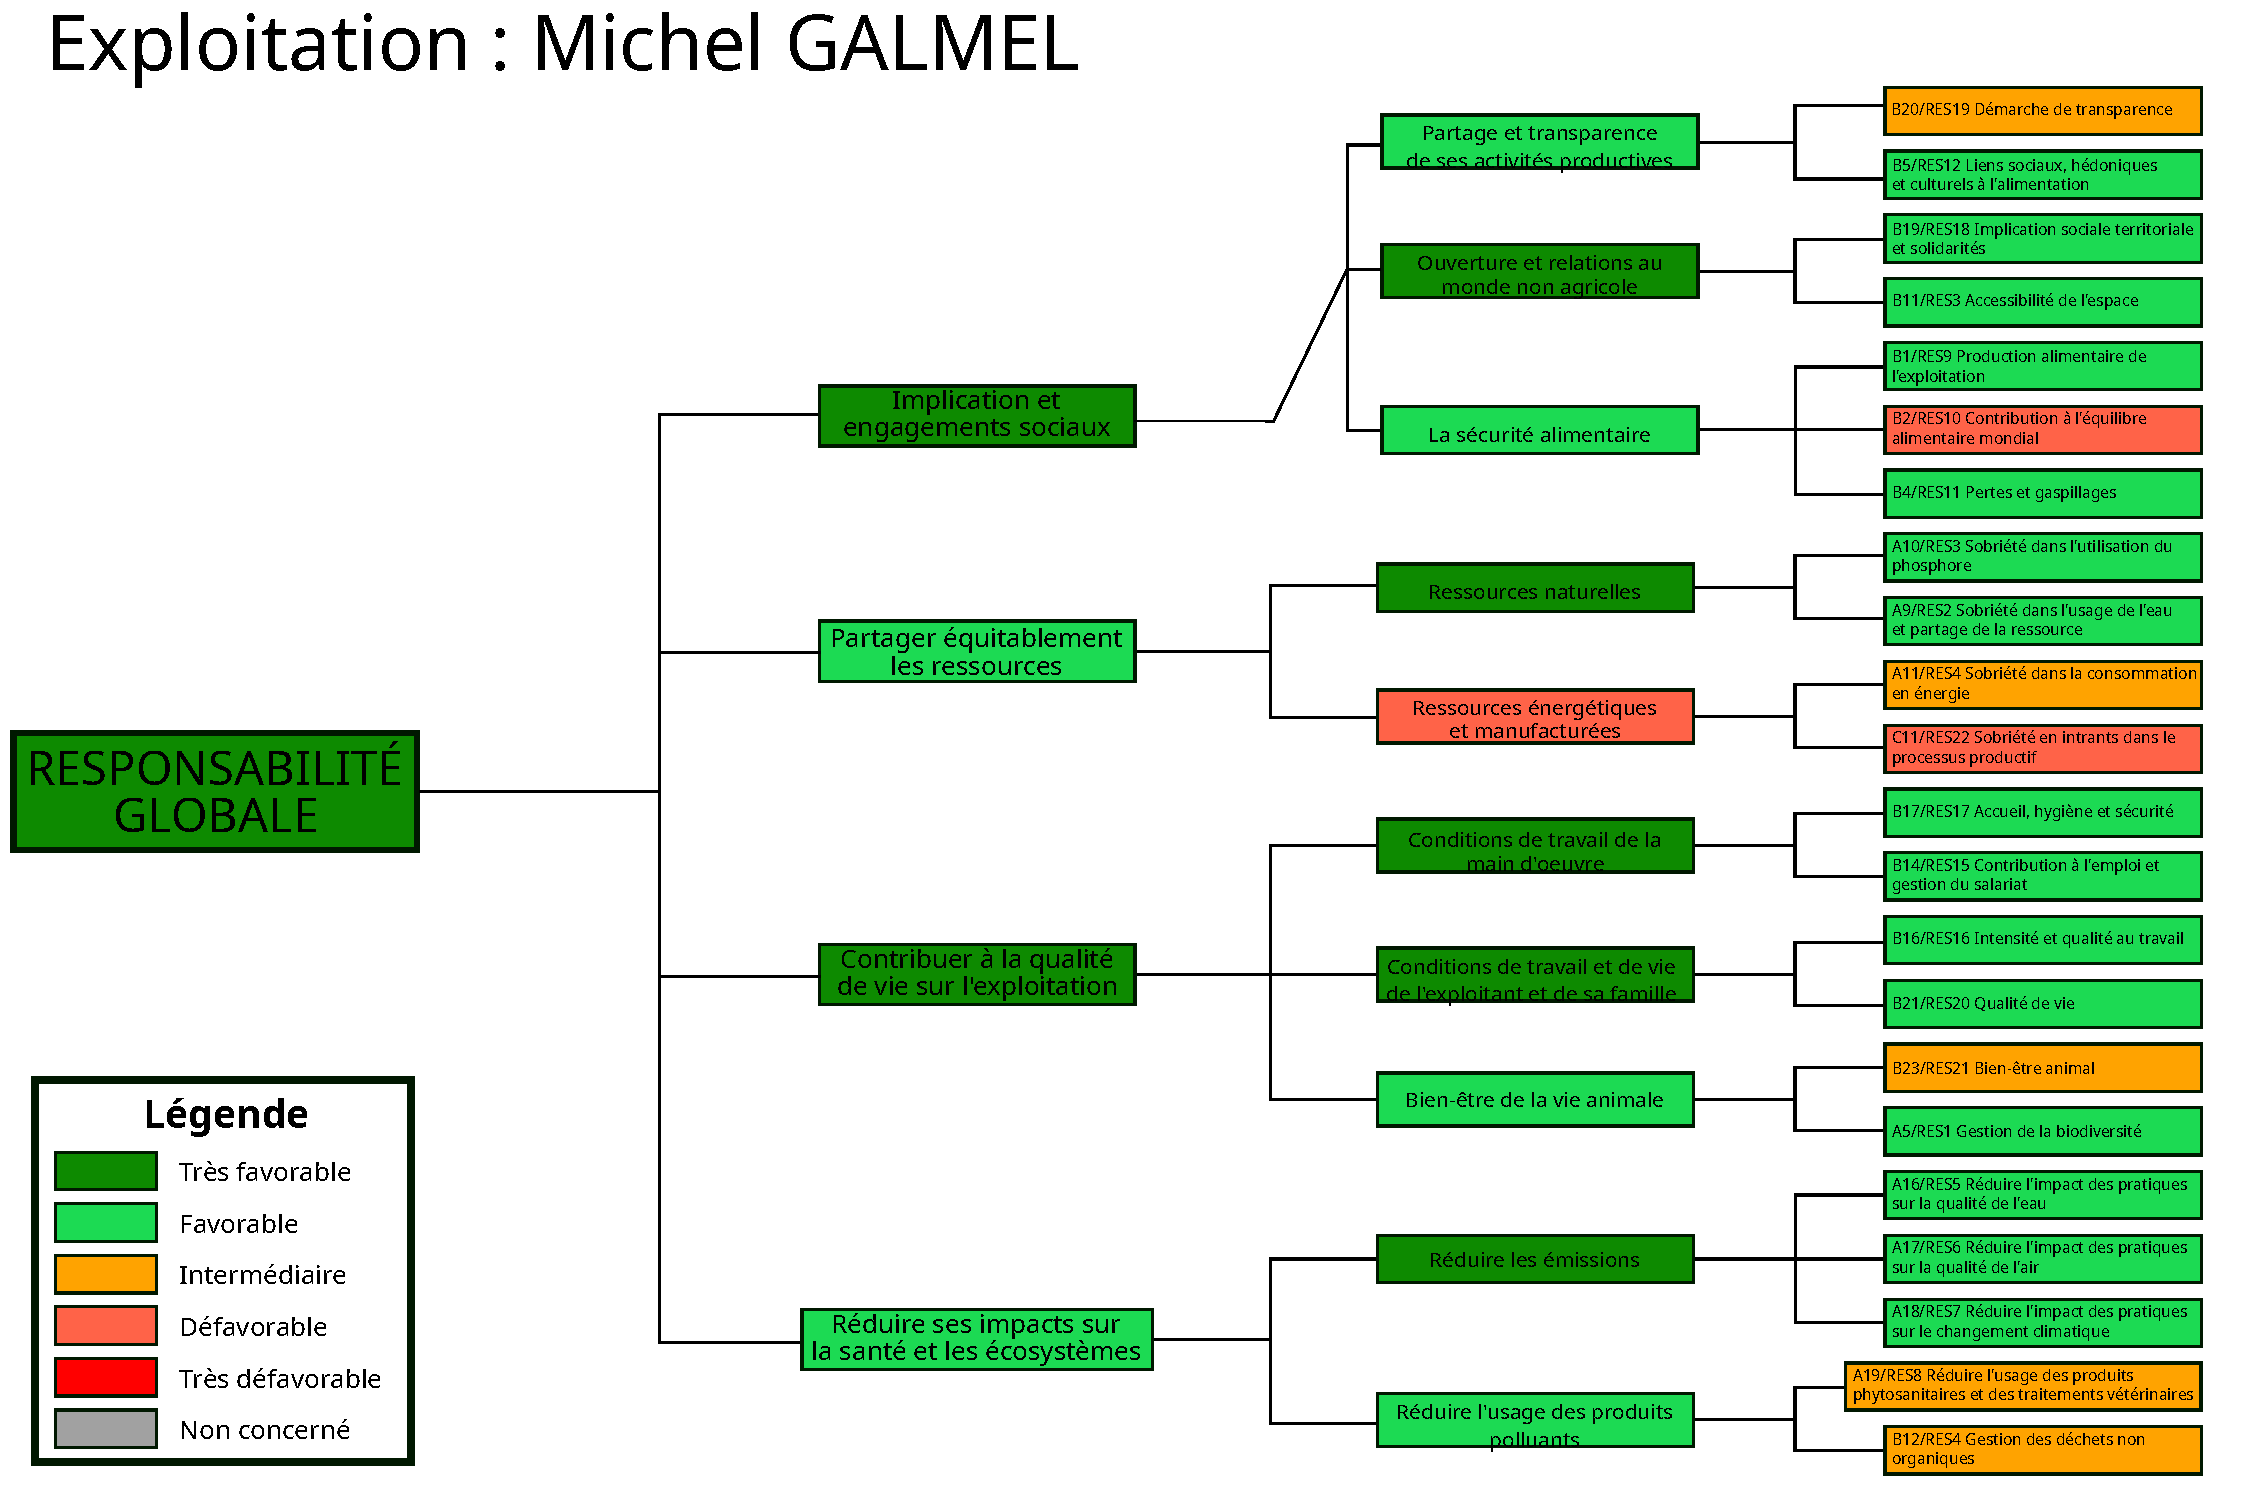
\includegraphics[width=1\linewidth]{/tmp/Rtmpy9IFHR/Michel_GALMEL/Propriétés/Cartes_heuristiques/Responsabilité} \caption{Responsabilité globale}\label{fig:unnamed-chunk-13}
\end{figure}
\end{minipage}}

\rotatebox{270}{
\begin{minipage}{\textheight}
\begin{figure}[H]
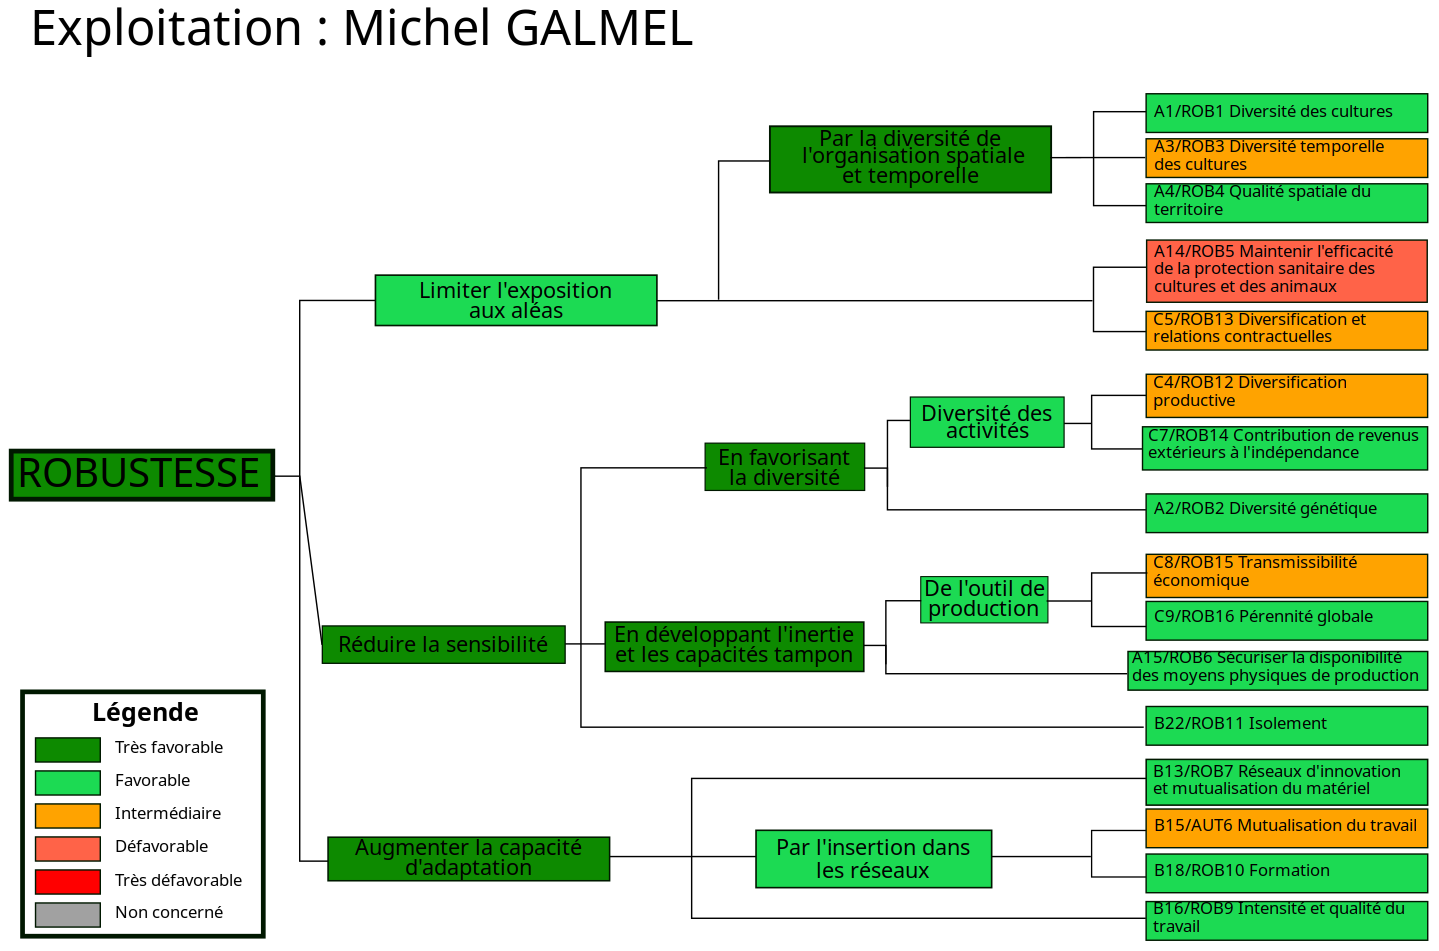
\includegraphics[width=1\linewidth]{/tmp/Rtmpy9IFHR/Michel_GALMEL/Propriétés/Cartes_heuristiques/Robustesse} \caption{Robustesse}\label{fig:unnamed-chunk-14}
\end{figure}
\end{minipage}}

\rotatebox{270}{
\begin{minipage}{\textheight}
\begin{figure}[H]
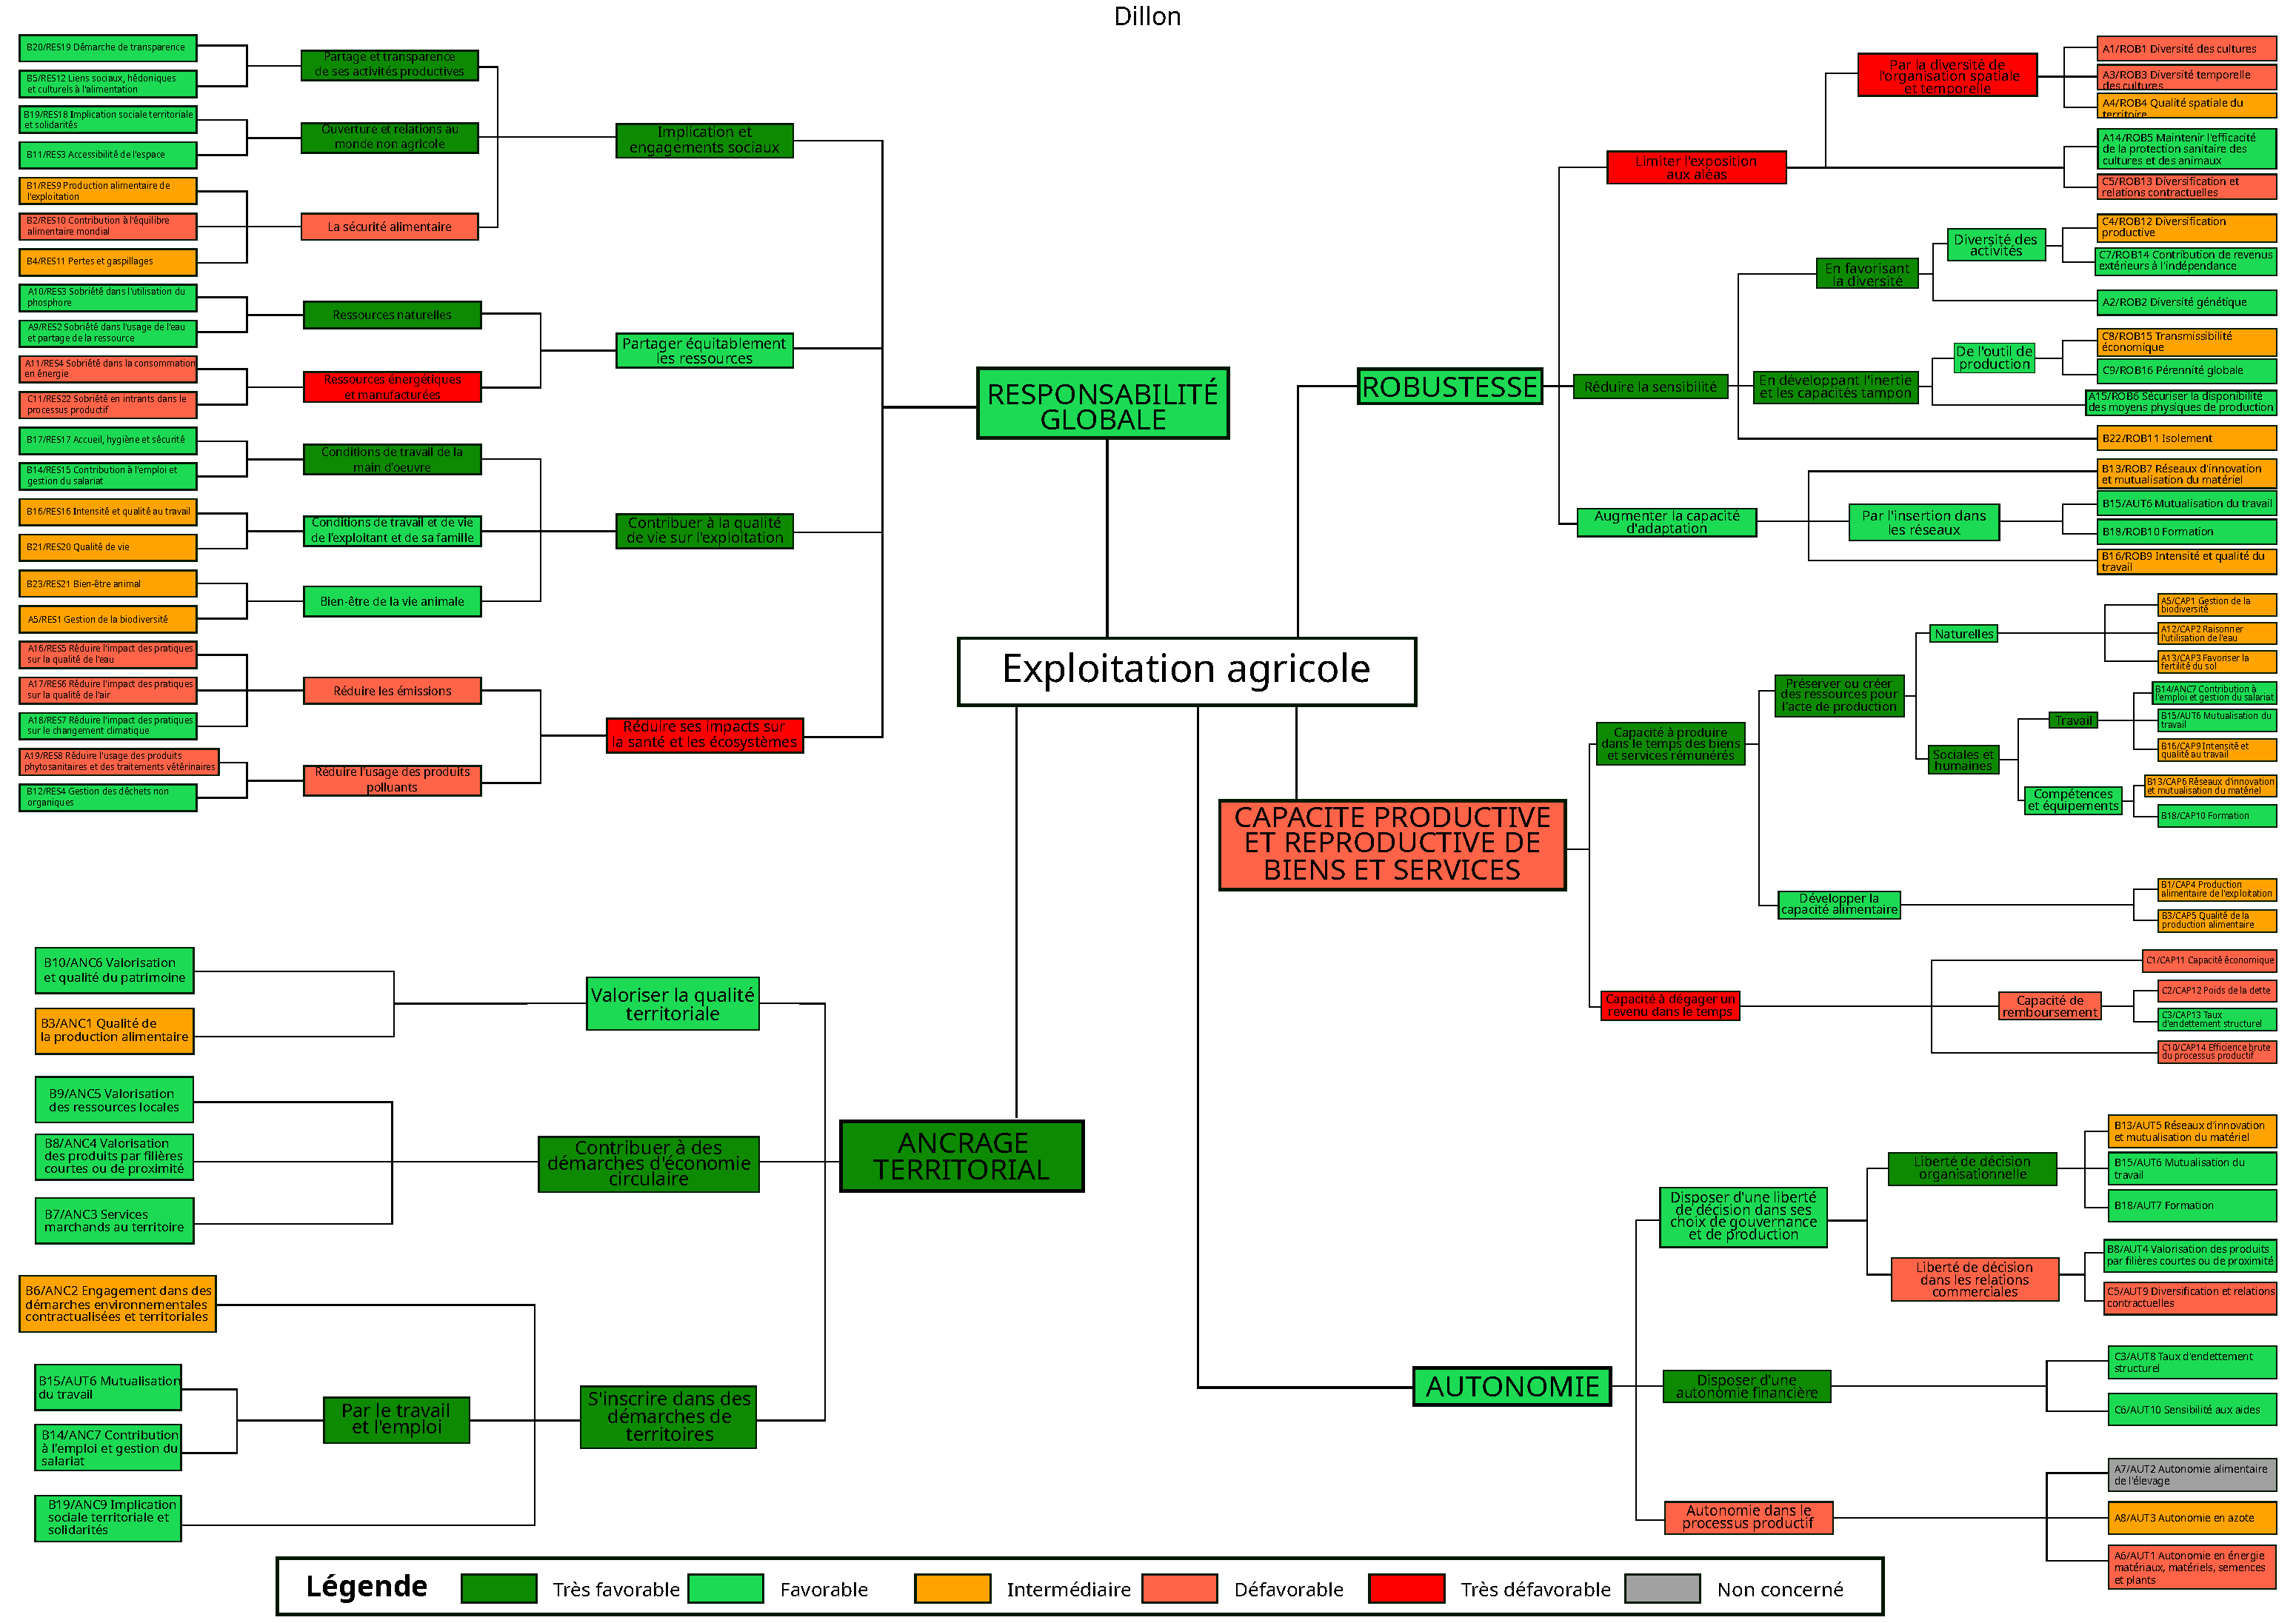
\includegraphics[width=1\linewidth]{/tmp/Rtmpy9IFHR/Michel_GALMEL/Propriétés/Cartes_heuristiques/Global} \caption{Vision globale de la lecture par les propriétés}\label{fig:unnamed-chunk-15}
\end{figure}
\end{minipage}}

\hypertarget{diagamme-radar-des-scores-obtenus-au-sein-de-chaque-propriuxe9tuxe9}{%
\subsection{Diagamme radar des scores obtenus au sein de chaque
propriété}\label{diagamme-radar-des-scores-obtenus-au-sein-de-chaque-propriuxe9tuxe9}}

\begin{figure}[H]

{\centering 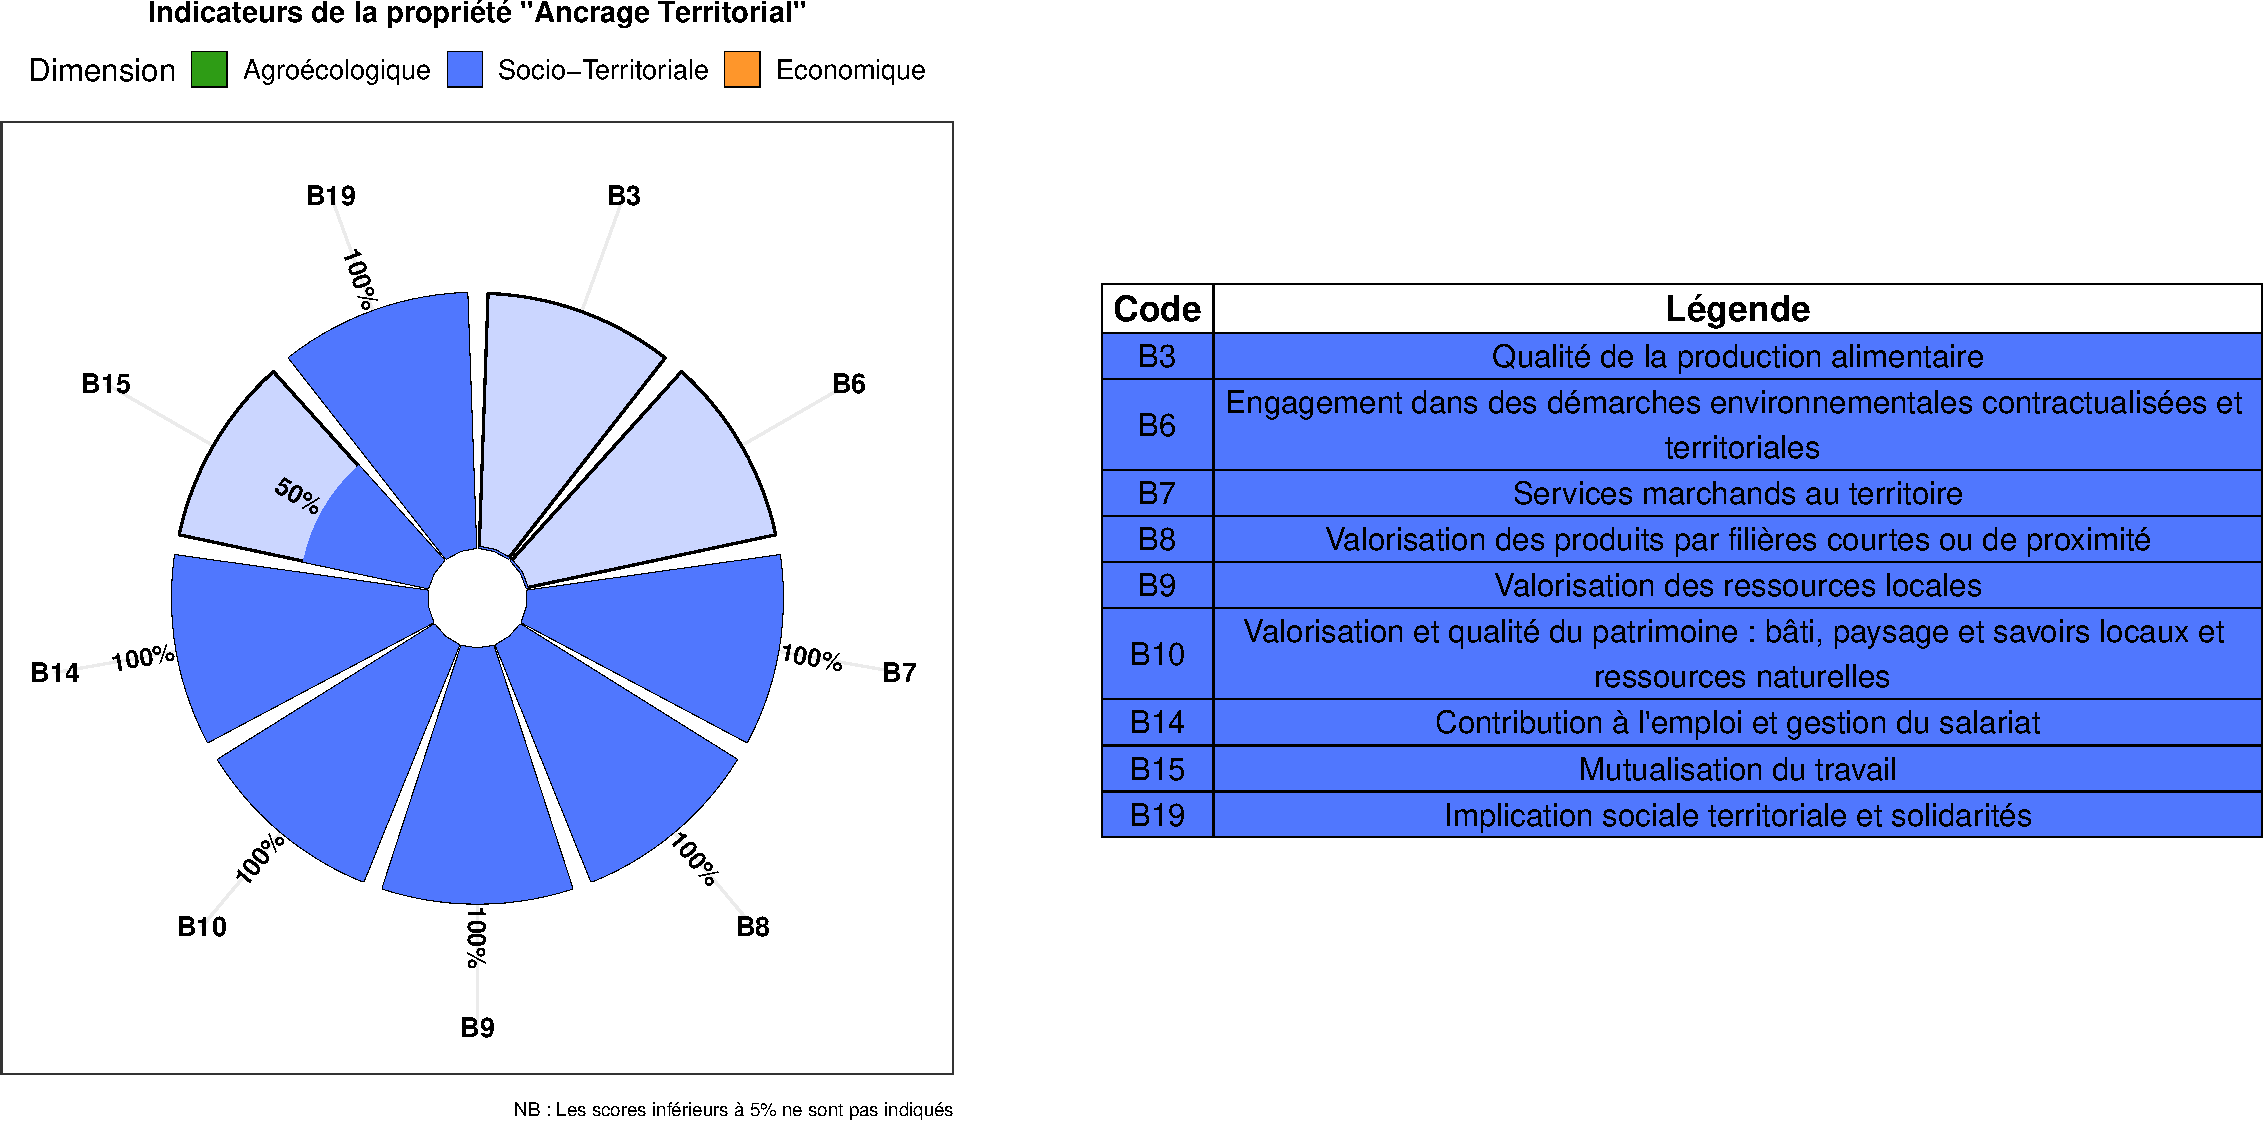
\includegraphics[width=1\linewidth]{report_files/figure-latex/unnamed-chunk-17-1} 

}

\caption{Pourcentage du score maximal obtenu pour chaque indicateur rattaché à la propriété Angrage territorial}\label{fig:unnamed-chunk-17}
\end{figure}

\begin{figure}[H]

{\centering 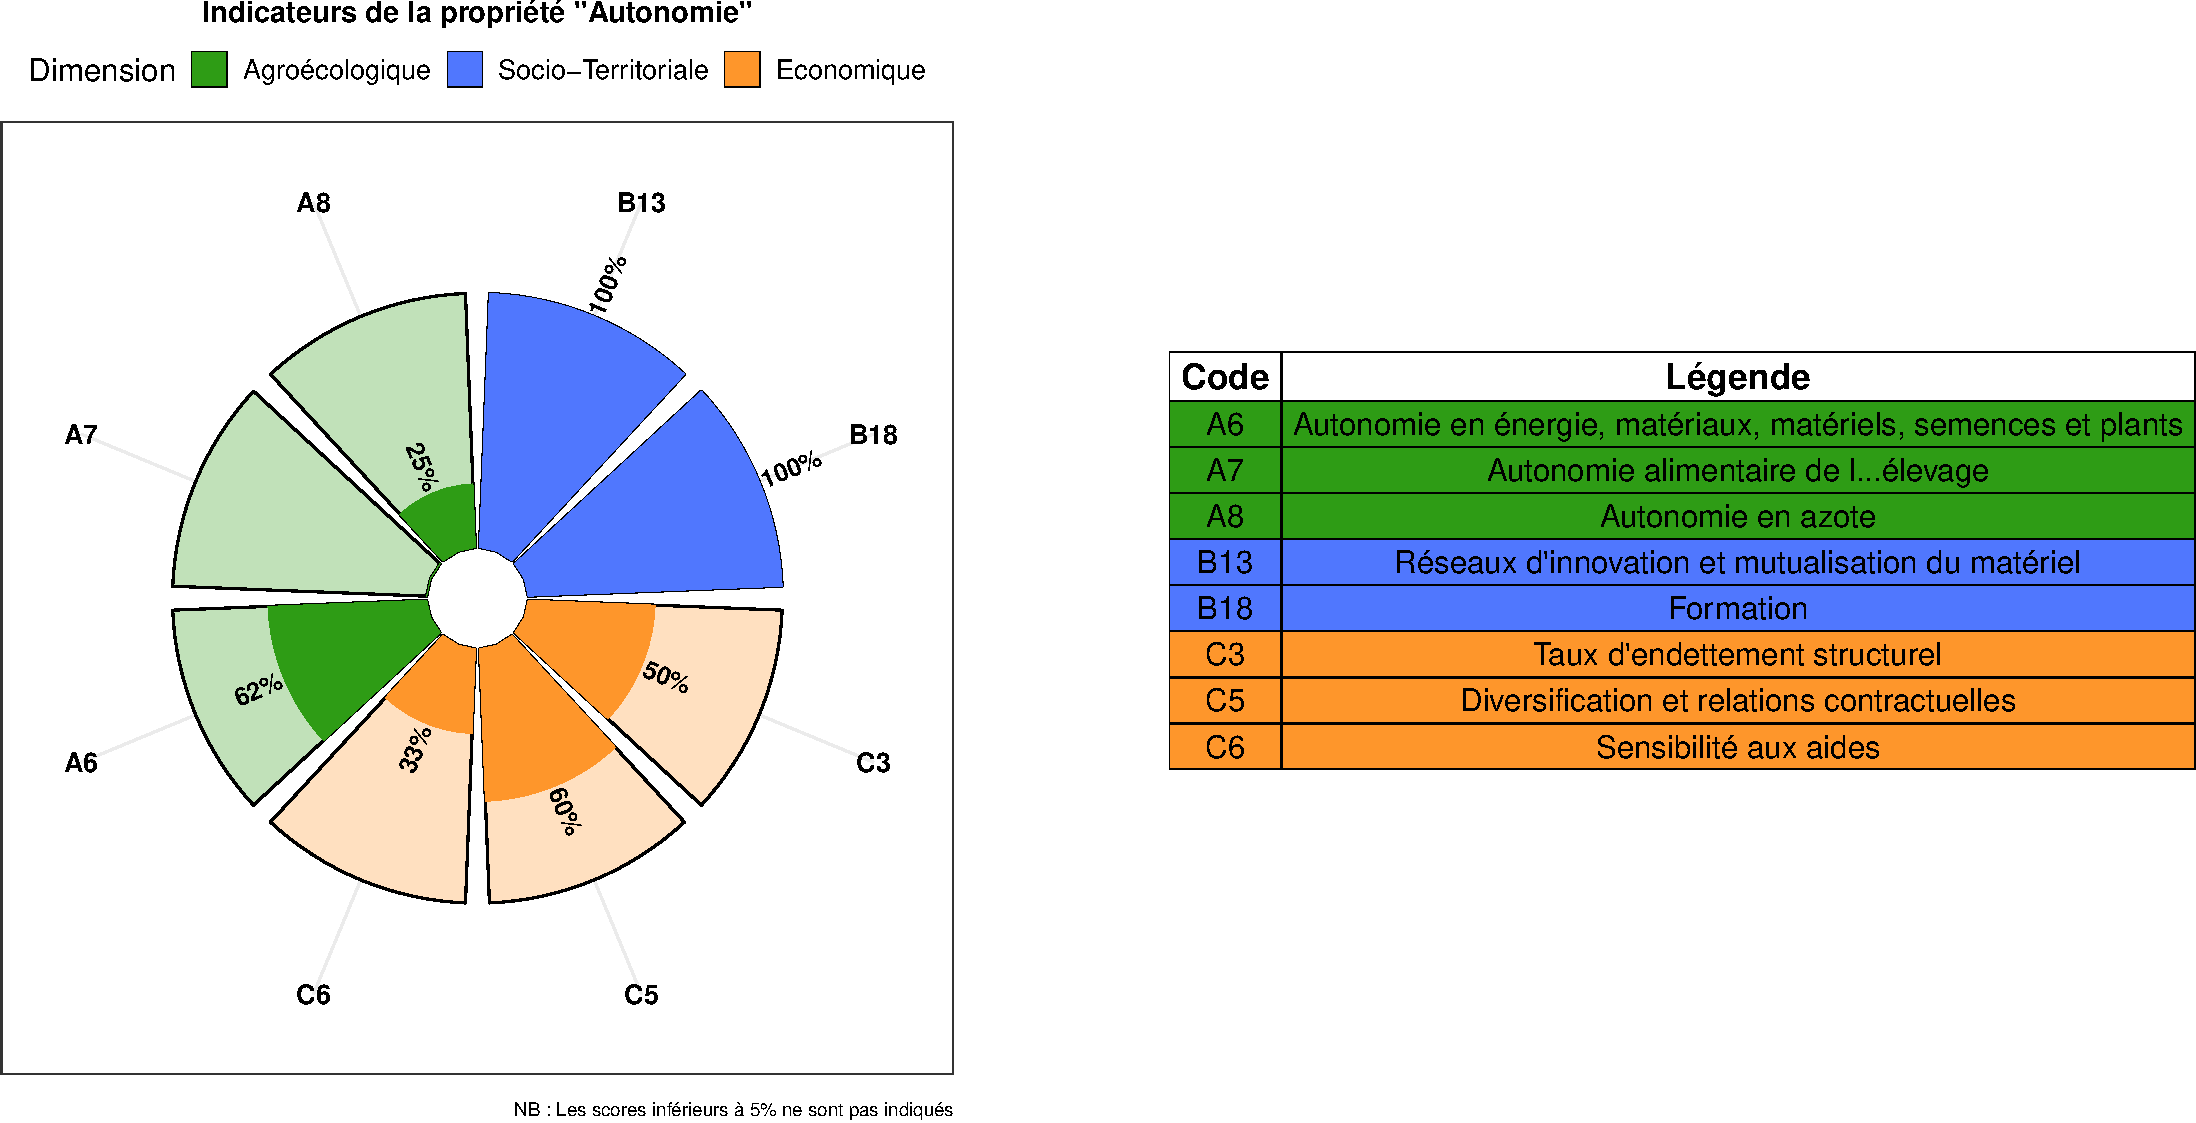
\includegraphics[width=1\linewidth]{report_files/figure-latex/unnamed-chunk-18-1} 

}

\caption{Pourcentage du score maximal obtenu pour chaque indicateur rattaché à la propriété Autonomie}\label{fig:unnamed-chunk-18}
\end{figure}

\begin{figure}[H]

{\centering 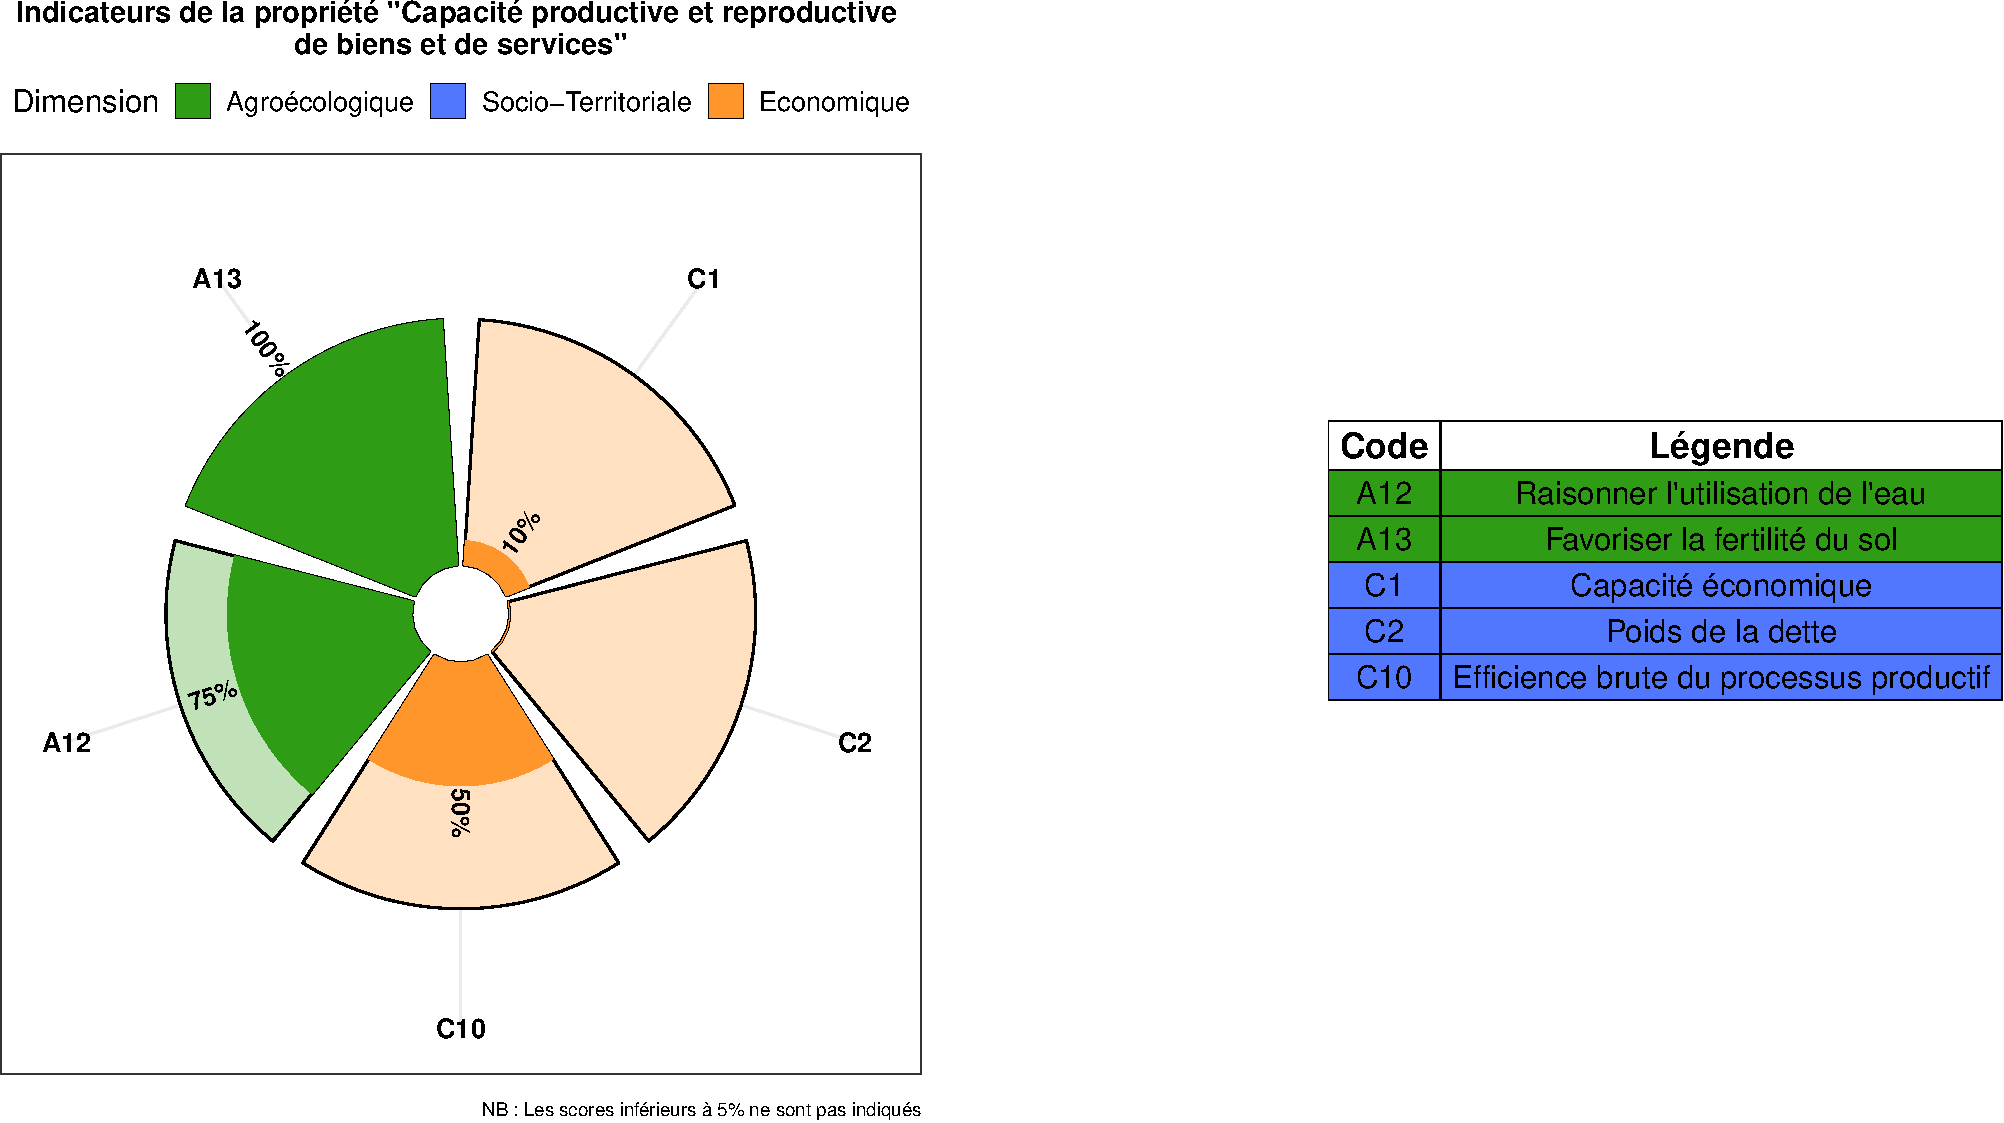
\includegraphics[width=1\linewidth]{report_files/figure-latex/unnamed-chunk-19-1} 

}

\caption{Pourcentage du score maximal obtenu pour chaque indicateur rattaché à la propriété Capacité productive et reproductive de biens et services}\label{fig:unnamed-chunk-19}
\end{figure}

\begin{figure}[H]

{\centering 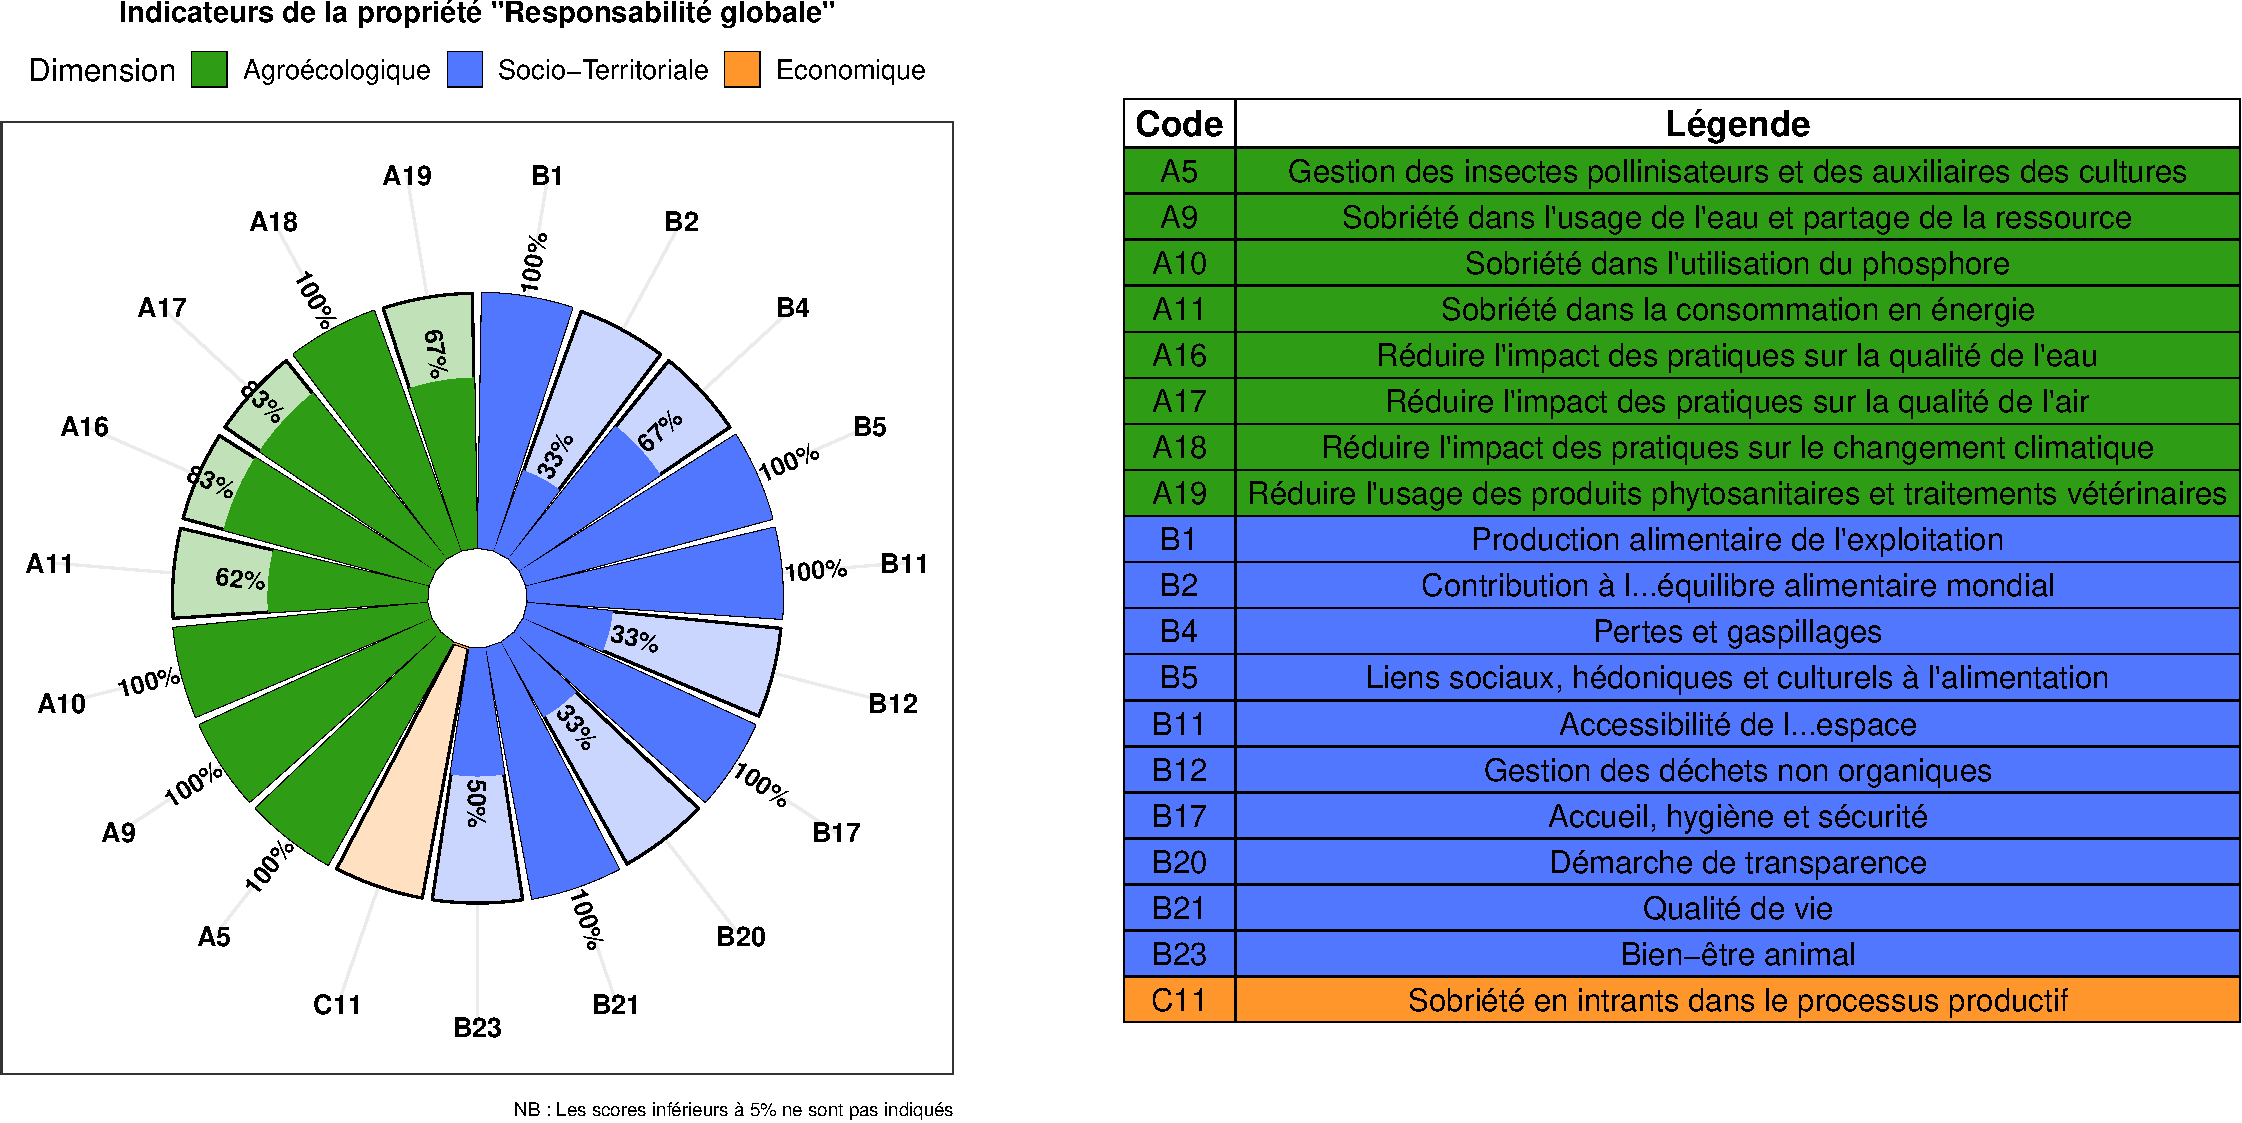
\includegraphics[width=1\linewidth]{report_files/figure-latex/unnamed-chunk-20-1} 

}

\caption{Pourcentage du score maximal obtenu pour chaque indicateur rattaché à la propriété Responsabilité globale}\label{fig:unnamed-chunk-20}
\end{figure}

\begin{figure}[H]

{\centering 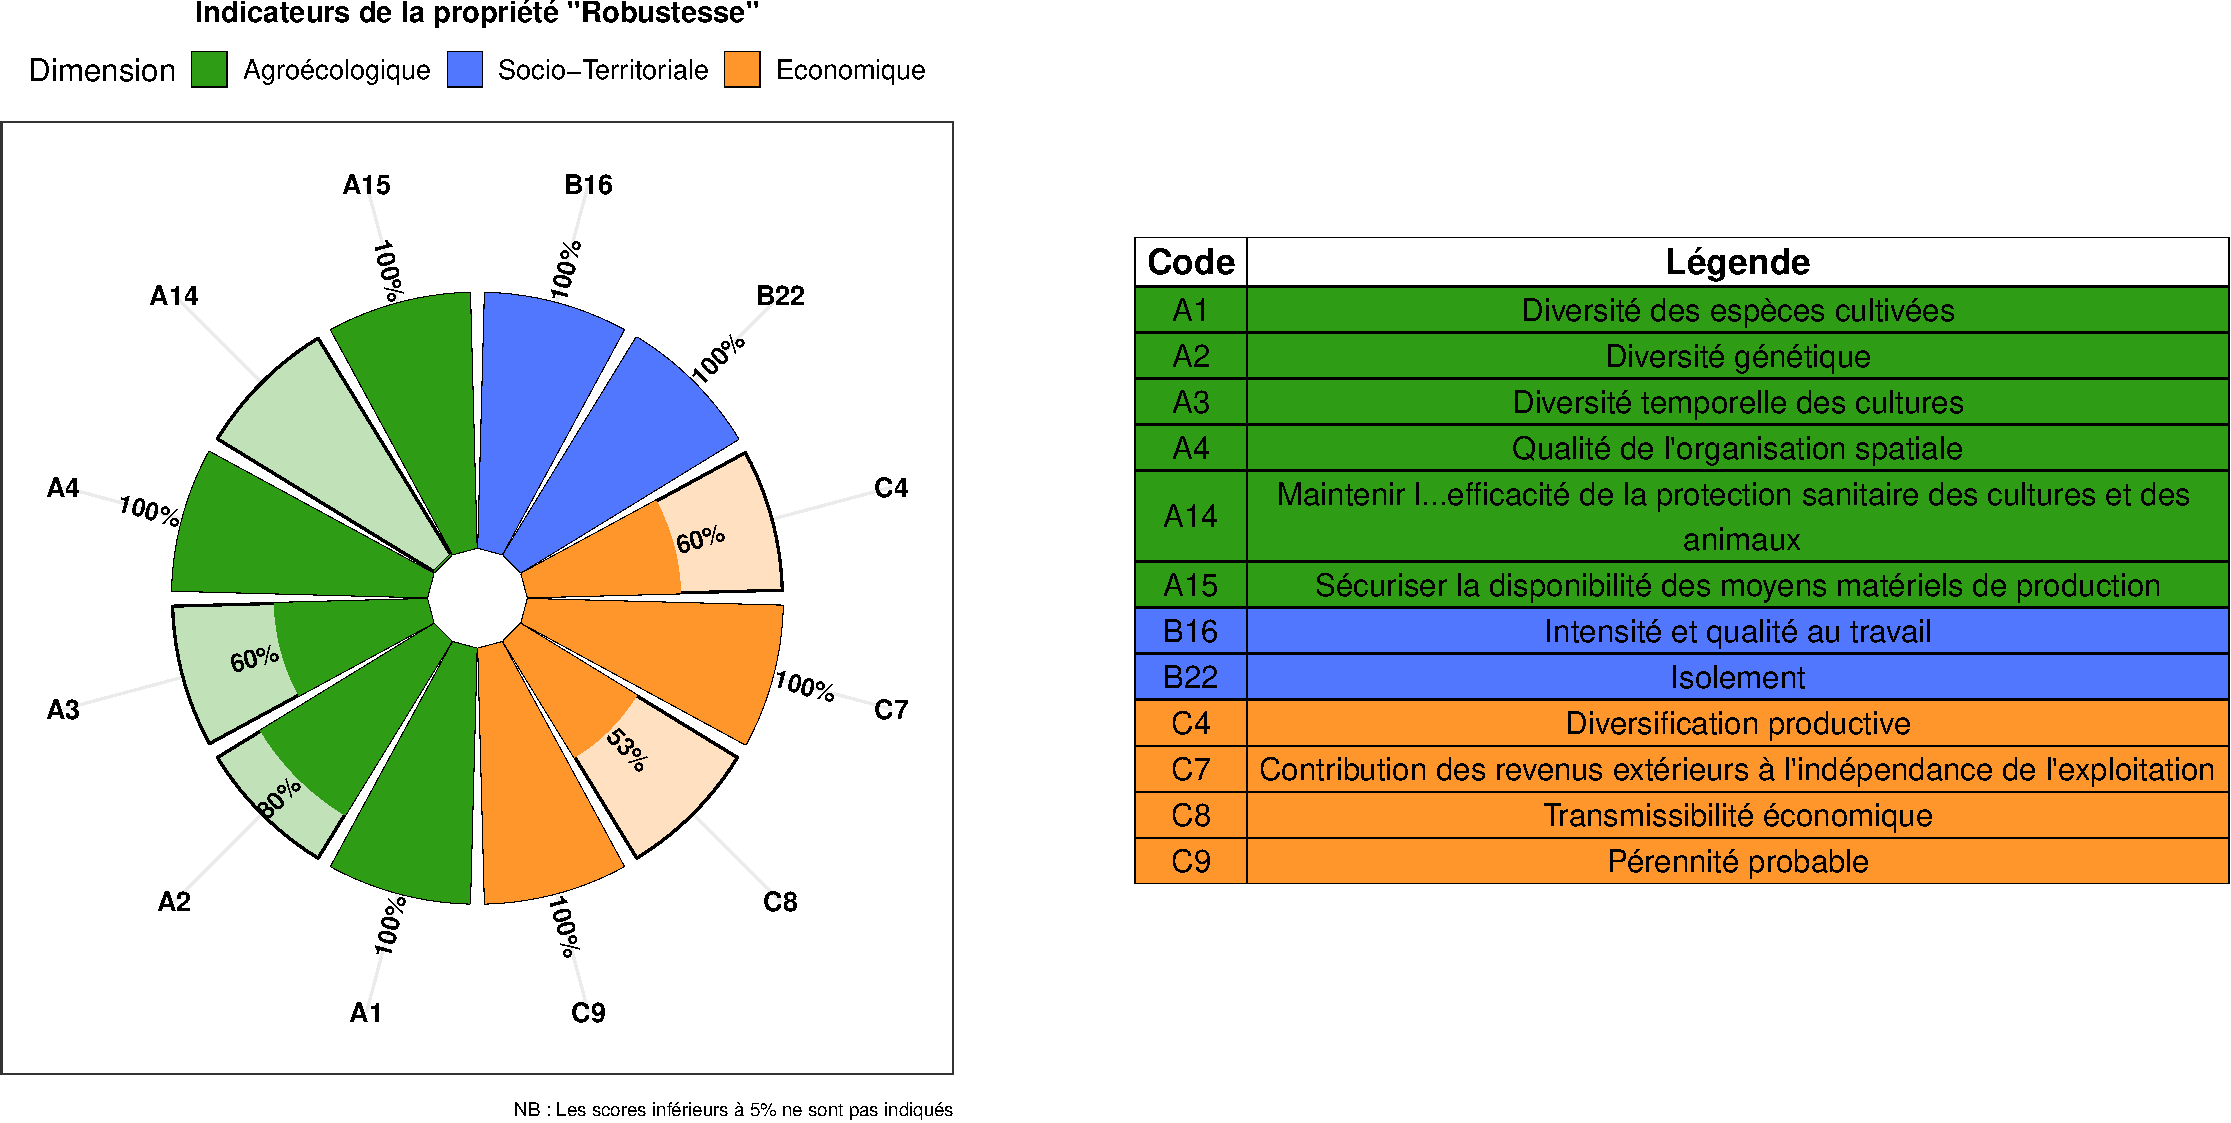
\includegraphics[width=1\linewidth]{report_files/figure-latex/unnamed-chunk-21-1} 

}

\caption{Pourcentage du score maximal obtenu pour chaque indicateur rattaché à la propriété Robustesse}\label{fig:unnamed-chunk-21}
\end{figure}

\newpage

\hypertarget{luxe9gende}{%
\section{Légende}\label{luxe9gende}}

\footnotesize

\begin{longtable}[]{@{}lll@{}}
\toprule
Code Indicateur & Nom Indicateur & Dimension\tabularnewline
\midrule
\endhead
A1 & Diversité des espèces cultivées & Durabilité
Agroécologique\tabularnewline
A2 & Diversité génétique & Durabilité Agroécologique\tabularnewline
A3 & Diversité temporelle des cultures & Durabilité
Agroécologique\tabularnewline
A4 & Qualité de l'organisation spatiale & Durabilité
Agroécologique\tabularnewline
A5 & Gestion des insectes pollinisateurs et des auxiliaires des cultures
& Durabilité Agroécologique\tabularnewline
A6 & Autonomie en énergie, matériaux, matériels, semences et plants &
Durabilité Agroécologique\tabularnewline
A7 & Autonomie alimentaire de l'élevage & Durabilité
Agroécologique\tabularnewline
A8 & Autonomie en azote & Durabilité Agroécologique\tabularnewline
A9 & Sobriété dans l'usage de l'eau et partage de la ressource &
Durabilité Agroécologique\tabularnewline
A10 & Sobriété dans l'utilisation du phosphore & Durabilité
Agroécologique\tabularnewline
A11 & Sobriété dans la consommation en énergie & Durabilité
Agroécologique\tabularnewline
A12 & Raisonner l'utilisation de l'eau & Durabilité
Agroécologique\tabularnewline
A13 & Favoriser la fertilité du sol & Durabilité
Agroécologique\tabularnewline
A14 & Maintenir l'efficacité de la protection sanitaire des cultures et
des animaux & Durabilité Agroécologique\tabularnewline
A15 & Sécuriser la disponibilité des moyens matériels de production &
Durabilité Agroécologique\tabularnewline
A16 & Réduire l'impact des pratiques sur la qualité de l'eau &
Durabilité Agroécologique\tabularnewline
A17 & Réduire l'impact des pratiques sur la qualité de l'air &
Durabilité Agroécologique\tabularnewline
A18 & Réduire l'impact des pratiques sur le changement climatique &
Durabilité Agroécologique\tabularnewline
A19 & Réduire l'usage des produits phytosanitaires et traitements
vétérinaires & Durabilité Agroécologique\tabularnewline
B1 & Production alimentaire de l'exploitation & Durabilité
Socio-Territoriale\tabularnewline
B2 & Contribution à l'équilibre alimentaire mondial & Durabilité
Socio-Territoriale\tabularnewline
B3 & Qualité de la production alimentaire & Durabilité
Socio-Territoriale\tabularnewline
B4 & Pertes et gaspillages & Durabilité
Socio-Territoriale\tabularnewline
B5 & Liens sociaux, hédoniques et culturels à l'alimentation &
Durabilité Socio-Territoriale\tabularnewline
B6 & Engagement dans des démarches environnementales contractualisées et
territoriales & Durabilité Socio-Territoriale\tabularnewline
B7 & Services marchands au territoire & Durabilité
Socio-Territoriale\tabularnewline
B8 & Valorisation des produits par filières courtes ou de proximité &
Durabilité Socio-Territoriale\tabularnewline
B9 & Valorisation des ressources locales & Durabilité
Socio-Territoriale\tabularnewline
B10 & Valorisation et qualité du patrimoine : bâti, paysage et savoirs
locaux et ressources naturelles & Durabilité
Socio-Territoriale\tabularnewline
B11 & Accessibilité de l'espace & Durabilité
Socio-Territoriale\tabularnewline
B12 & Gestion des déchets non organiques & Durabilité
Socio-Territoriale\tabularnewline
B13 & Réseaux d'innovation et mutualisation du matériel & Durabilité
Socio-Territoriale\tabularnewline
B14 & Contribution à l'emploi et gestion du salariat & Durabilité
Socio-Territoriale\tabularnewline
B15 & Mutualisation du travail & Durabilité
Socio-Territoriale\tabularnewline
B16 & Intensité et qualité au travail & Durabilité
Socio-Territoriale\tabularnewline
B17 & Accueil, hygiène et sécurité & Durabilité
Socio-Territoriale\tabularnewline
B18 & Formation & Durabilité Socio-Territoriale\tabularnewline
B19 & Implication sociale territoriale et solidarités & Durabilité
Socio-Territoriale\tabularnewline
B20 & Démarche de transparence & Durabilité
Socio-Territoriale\tabularnewline
B21 & Qualité de vie & Durabilité Socio-Territoriale\tabularnewline
B22 & Isolement & Durabilité Socio-Territoriale\tabularnewline
B23 & Bien-être animal & Durabilité Socio-Territoriale\tabularnewline
C1 & Capacité économique & Durabilité Economique\tabularnewline
C2 & Poids de la dette & Durabilité Economique\tabularnewline
C3 & Taux d'endettement structurel & Durabilité
Economique\tabularnewline
C4 & Diversification productive & Durabilité Economique\tabularnewline
C5 & Diversification et relations contractuelles & Durabilité
Economique\tabularnewline
C6 & Sensibilité aux aides & Durabilité Economique\tabularnewline
C7 & Contribution des revenus extérieurs à l'indépendance de
l'exploitation & Durabilité Economique\tabularnewline
C8 & Transmissibilité économique & Durabilité Economique\tabularnewline
C9 & Pérennité probable & Durabilité Economique\tabularnewline
C10 & Efficience brute du processus productif & Durabilité
Economique\tabularnewline
C11 & Sobriété en intrants dans le processus productif & Durabilité
Economique\tabularnewline
\bottomrule
\end{longtable}

\end{document}
